% \documentclass[a4paper,10pt]{article}

% \usepackage[a4paper, margin=1in]{geometry} % Set 1 inch margins (adjust as needed)
% \usepackage{tikz,tikz-3dplot}
% \usepackage{subcaption}
% \usepackage{hyperref}
% \usepackage{algorithm2e}
% \usepackage{graphicx}
% \usepackage{listings}
% \usetikzlibrary{trees}

% \lstdefinestyle{BashInputStyle}{
%   language=bash,
%   basicstyle=\small\ttfamily,
% %  numbers=left,
% %  numberstyle=\tiny,
% %  numbersep=3pt,
%   frame=single,
%   columns=fullflexible,
%   backgroundcolor=\color{yellow!10},
%   linewidth=0.95\linewidth,
%   xleftmargin=0.05\linewidth,
%   keepspaces=true,
%   breaklines=true,
%   framesep=5pt,
%   rulecolor=\color{black!30},
%   aboveskip=10pt,
% }

% \begin{document}

\section{Introduction}
NekMesh is described in its paper \cite{NekMesh_paper} as "an
open-source mesh generation package which is designed to enable the
generation of valid, high-quality curvilinear meshes of complex,
three-dimensional geometries for performing high-order simulations."
To summarise, NekMesh is comprised of various Input, Process and
Output modules, and the workflow is to run 1) one input module 2) $n$
process modules 3) one output module. Before learning about the three
module types, we need a good understanding of the theory underpinning
the NekMesh format.

\section{Overview of the redesign}
\label{sect:redesign_overview}
This section describes the ongoing redesign of NekMesh relative to the
\texttt{master} branch. It is intended as an orientation guide for
developers who know the old code base and need to understand what has
moved, what has been ported, and what is temporarily disabled. The
subsequent sections of this document describe the design as it now
stands.

\subsection{Motivation}
Historically NekMesh maintained its \textit{own} mesh data structures
(\texttt{Node}, \texttt{Edge}, \texttt{Face}, \texttt{Element},
\texttt{Composite}) which duplicated, but were not interoperable with,
the \texttt{SpatialDomains} geometry objects (\texttt{PointGeom},
\texttt{SegGeom}, \texttt{TriGeom}/\texttt{QuadGeom},
\texttt{TetGeom}, \texttt{PrismGeom}, \ldots) used by the solvers. Every
NekMesh run therefore ended in a translation step: the NekMesh
representation was converted into geometry objects (or serialised to
XML) before it could be used. This had three consequences:

\begin{enumerate}
  \item \textbf{Duplication.} Connectivity, curvature and
    high-order node handling were implemented twice, in two
    conventions that had to be kept in sync.
  \item \textbf{Cost.} Large industrial meshes were held twice in
    memory, and the conversion between representations dominated the
    runtime of several modules.
  \item \textbf{No pipelining.} Because NekMesh objects were not
    geometry objects, a mesh could not be handed straight to a solver,
    nor could a solver-side \texttt{MeshGraph} be fed back into a
    process module.
\end{enumerate}

The redesign removes the duplication by making
\texttt{SpatialDomains} the single mesh representation: NekMesh now
\textit{operates directly on} a \texttt{MeshGraph}. This enables an
in-memory, MPI-parallel meshing pipeline (mesh $\rightarrow$ process
$\rightarrow$ solve) without file round-trips.

\subsection{Summary of the data structure changes}
\label{sect:ds_summary}
Table \ref{tab:ds_mapping} maps each of the old NekMesh structures onto
its replacement. The rest of this section explains each entry in turn.

\begin{table}[h!]
  \centering
  \begin{tabular}{p{0.28\textwidth}p{0.32\textwidth}p{0.30\textwidth}}
    \hline
    \textbf{Was} & \textbf{Is now} & \textbf{Note}\\
    \hline
    \texttt{NodeSharedPtr} &
    \texttt{SpatialDomains::PointGeom*} &
    owned by the graph, passed by raw pointer\\
    \texttt{EdgeSharedPtr} &
    \texttt{SpatialDomains::SegGeom*} &
    \texttt{Edge.cpp/.h} out of the build\\
    \texttt{FaceSharedPtr} &
    \texttt{SpatialDomains::Geometry2D*} &
    \texttt{Face.cpp/.h} out of the build\\
    \texttt{Element} (owns nodes) &
    \texttt{Geometry}/\texttt{Geometry2D}/\texttt{Geometry3D} &
    \texttt{Element} is now only a shape-level builder\\
    \texttt{Mesh::m\_node}, \texttt{m\_vertexSet}, \texttt{m\_numNodes} &
    \texttt{MeshGraph} point-geometry map &
    \texttt{GetGeomMap<PointGeom>()}\\
    \texttt{Mesh::m\_element} (\texttt{ElementMap}) &
    \texttt{MeshGraph} per-shape geometry maps &
    \texttt{GetGeomMap<T>()}, keyed by global ID\\
    \texttt{Mesh::m\_composite} (\texttt{CompositeMap}) &
    \texttt{Mesh::m\_elementTags} &
    \texttt{array<unordered\_map<Geometry*,int>,4>}\\
    \texttt{Mesh::m\_edgeSet}, \texttt{m\_faceSet}
    (\texttt{EdgeSet}/\texttt{FaceSet} of shared pointers) &
    \texttt{EdgeMap}, \texttt{FaceMap}
    (hash maps to \texttt{SegGeom*}/\texttt{Geometry2D*}) &
    same hashing, non-owning\\
    \texttt{Mesh::m\_expDim}, \texttt{m\_spaceDim} &
    \texttt{MeshGraph::GetMeshDimension()},
    \texttt{GetSpaceDimension()} &
    dimensions live with the graph\\
    \texttt{Mesh::m\_cad} &
    \texttt{MeshGraph} / \texttt{SpatialDomains::CADSystem} &
    see the CAD subsection below\\
    (no equivalent) &
    \texttt{SpatialDomains::EntityHolder} &
    owns geometry not yet in the graph\\
    (no equivalent) &
    \texttt{ElmtIds} &
    explicit, deterministic IDs on creation\\
    \hline
  \end{tabular}
  \caption{Correspondence between the old NekMesh mesh structures and
    the new \texttt{SpatialDomains}-based ones.}
  \label{tab:ds_mapping}
\end{table}

The changes fall into four groups, in decreasing order of impact on
calling code:

\begin{enumerate}
  \item \textbf{Representation.} Nodes, edges, faces and elements are
    now geometry objects. Any code that dereferenced
    \texttt{node->m\_x} or iterated \texttt{el->GetVertexList()} must
    be rewritten against the \texttt{Geometry} interface.
  \item \textbf{Ownership.} The \texttt{MeshGraph} owns every entity
    through \texttt{unique\_ptr\_objpool}; everybody else holds raw
    pointers. Shared-pointer reference counting no longer keeps
    entities alive, so lifetime is now explicit.
  \item \textbf{Identity.} Entities are addressed by global ID within
    the graph's maps rather than by pointer identity within a set, and
    IDs can be pinned at creation.
  \item \textbf{Grouping.} Composites are replaced by a
    geometry-to-tag map, one per dimension.
\end{enumerate}

\subsection{The single data structure}
The central change is in \texttt{MeshElements/Mesh.h}. The old
\texttt{Mesh} class owned \texttt{m\_node}, \texttt{m\_vertexSet},
\texttt{m\_element}, \texttt{m\_composite} and friends. The new
\texttt{Mesh} owns essentially one thing:

\begin{lstlisting}[style=BashInputStyle]
class Mesh
{
public:
    /// Mesh graph shared ptr storing the geometry info
    SpatialDomains::MeshGraphSharedPtr m_meshGraph;
    /// Array by dimension of maps of all elements and boundary
    /// surfaces to their tags.
    std::array<GeomTagMap, 4> m_elementTags;
    /// Map of element edges / faces.
    EdgeMap m_edgeSet;
    FaceMap m_faceSet;
    ...
    /// Information handed from one module to another.
    ModuleContext &GetContext();
private:
    ModuleContext m_context;
};
\end{lstlisting}

Taking each member in turn:

\begin{itemize}
  \item \textbf{\texttt{m\_meshGraph} --- the \texttt{MeshGraph} owns
    the mesh.} Geometry objects are held by the graph in per-shape
    maps (\texttt{m\_pointGeoms}, \texttt{m\_segGeoms},
    \texttt{m\_triGeoms}, \ldots) of \texttt{unique\_ptr\_objpool},
    keyed by global ID; everything else refers to them by \textit{raw
    pointer}. This replaces both \texttt{m\_node}/\texttt{m\_vertexSet}
    and \texttt{m\_element}. Ownership is transferred explicitly
    through the new \texttt{MeshGraph} API:

    \begin{itemize}
      \item \texttt{AddGeom<T>(id, geom)} --- hand a single entity to
        the graph. The type-dispatched overload for \texttt{T =
        Geometry} switches on \texttt{GetShapeType()} and downcasts,
        so a module holding a generic \texttt{Geometry} need not know
        the concrete shape.
      \item \texttt{BulkAddGeom<T>(vector)} --- move a whole batch in
        at once, which avoids repeated map rehashing when a module
        creates many entities (e.g. boundary-layer splitting).
      \item \texttt{ExtractGeom<T>(id, erase)} --- take ownership
        \textit{back} out of the graph, optionally erasing the map
        entry. This is how a module temporarily removes entities it is
        about to replace.
      \item \texttt{GetGeomMap<T>()} / \texttt{SetGeomMap<T>()} ---
        read or wholesale-replace a shape's map; the latter is used
        when renumbering.
    \end{itemize}

    Insertion goes through \texttt{InsertGeomChecked}, which asserts
    that the ID is not already present, so a duplicate global ID is now
    a hard error rather than silent corruption of the mesh.

  \item \textbf{\texttt{m\_elementTags} --- composites replaced by
    tags.} \texttt{m\_elementTags[dim]} is a
    \texttt{unordered\_map<Geometry*, int>} (\texttt{GeomTagMap})
    associating each geometry of that dimension with its
    composite/tag. The old \texttt{CompositeMap} was the inverse
    relation --- tag $\rightarrow$ list of elements --- which meant a
    linear search to answer "which composite is this element in?", the
    question modules actually ask. Boundary membership is now a single
    lookup, \texttt{Mesh::IsBoundary(geom, dim)}. Note that an entity
    carries a single \texttt{int} tag rather than a
    \texttt{vector<int>}. The counting helpers follow:
    \texttt{GetNumEntities()} has become
    \texttt{GetNumTaggedEntities()}.

  \item \textbf{\texttt{m\_edgeSet}, \texttt{m\_faceSet} ---
    connectivity lookup.} These retain their old purpose (find the
    existing edge/face defined by a given set of vertex IDs, so that
    neighbouring elements share it rather than duplicating it) and
    their old hashing, but they are now non-owning maps to geometry
    pointers:
\begin{lstlisting}[style=BashInputStyle]
typedef std::unordered_map<std::pair<int,int>,
        SpatialDomains::SegGeom*, EdgeHash, EdgeKey>    EdgeMap;
typedef std::unordered_map<std::array<int,4>,
        SpatialDomains::Geometry2D*, FaceHash, FaceKey> FaceMap;
\end{lstlisting}
    \texttt{EdgeHash}/\texttt{EdgeKey} hash an edge on its two vertex
    IDs irrespective of order; \texttt{FaceHash}/\texttt{FaceKey} do
    the same for the (up to) four vertex IDs of a face via the
    \texttt{sort4} sorting network. A face key is a fixed
    \texttt{array<int,4>}, with triangles using the fourth slot as a
    sentinel.

  \item \textbf{What disappeared.} \texttt{Node}, \texttt{Edge},
    \texttt{Face}, \texttt{Point}, \texttt{Composite},
    \texttt{HOAlignment} and \texttt{Pyramid} are commented out of
    \texttt{library/NekMesh/CMakeLists.txt} (the files remain on disk
    for reference only). \texttt{m\_expDim} and \texttt{m\_spaceDim}
    move to \texttt{MeshGraph::GetMeshDimension()} and
    \texttt{GetSpaceDimension()}. \texttt{m\_cad} moves into
    \texttt{SpatialDomains}. The auxiliary members
    \texttt{m\_vertexNormals}, \texttt{m\_spherigonSurfs},
    \texttt{m\_faceLabels}, \texttt{m\_condition} and \texttt{m\_fields}
    are not carried over as members: those still needed are now
    module-to-module payloads held in the \texttt{ModuleContext}
    described below, rather than fields on \texttt{Mesh} that every
    module pays for and no module owns. (The \texttt{Condition} type
    itself is still declared in \texttt{Mesh.h}.)
\end{itemize}

\subsubsection{ModuleContext --- payloads between modules}
\texttt{NekMesh.cpp} builds a pipeline of modules and runs them in
sequence, and some of them need to hand something to a later one that
is not mesh data: vertex normals read from a \texttt{.ply} file and
consumed by the spherigon module, the octree built by
\texttt{loadoctree} and used by surface meshing, the coarse elements
\texttt{ProcessBL} keeps so that a boundary layer can later be
regenerated. Historically each of these was a member of \texttt{Mesh}
(\texttt{m\_vertexNormals}, \texttt{m\_octree},
\texttt{m\_macroElements}, \ldots), which put single-module concerns in
the one class every module includes, and gave the payload no clear
owner or lifetime.

\texttt{ModuleContext} (\texttt{NekMesh/Module/ModuleContext.h}),
reached through \texttt{Mesh::GetContext()}, is a store keyed on the
payload's own type:

\begin{lstlisting}[style=BashInputStyle]
// Producer, in the module that has the information:
m_mesh->GetContext().Get<VertexNormals>().normals[vert] = {nx, ny, nz};

// Consumer, in a module that may or may not be given it:
if (VertexNormals *vn = m_mesh->GetContext().TryGet<VertexNormals>())
{
    ...
}
\end{lstlisting}

\noindent \texttt{Set<T>} replaces a payload, \texttt{Get<T>}
constructs one if absent or stale, \texttt{TryGet<T>} returns
\texttt{nullptr} in that case instead, and \texttt{Remove<T>} drops
one. The distinction matters to a consumer that must tell ``nothing was
supplied'' from ``something was supplied and is empty'', which a
\texttt{size() == 0} test cannot do. The key is
\texttt{std::type\_index}, so there are no string names
to keep in sync and a typo is a compile error; entries are held as
\texttt{shared\_ptr<void>}, which (unlike \texttt{unique\_ptr<void>} or
\texttt{std::any}) retains the concrete deleter, so the payload type
need only be complete where it is used.

The payload types themselves are small structs declared next to the
context: \texttt{VertexNormals} and \texttt{SpherigonSurfs}
(\texttt{Module/SurfaceHints.h}) and \texttt{MacroElements}
(\texttt{Module/MacroElements.h}), the last of which wraps an
\texttt{EntityHolder} --- a plain owning container of unique pointers,
one vector per geometry type, for entities that must stay alive while
not part of the graph.

\paragraph{Staleness.} A payload that refers to mesh entities is
invalidated when those entities may have gone.
\texttt{Module::RemoveOrphanedEntities()} calls
\texttt{ModuleContext::Invalidate()}, which bumps a generation counter;
\texttt{TryGet<T>} compares generations and reports a payload stored
before the last invalidation as absent. This is deliberately coarse ---
``the mesh changed, discard'' --- because testing whether a particular
entity survived would cost more than rebuilding the payload.
Renumbering, by contrast, is deliberately \textit{not} an invalidation:
keying a payload on geometry pointers rather than on global IDs is
precisely what lets it survive one.

Not every payload wants that, and the trait
\texttt{PayloadFollowsEntities<T>} says so. It defaults to
\texttt{true\_type}, the safe answer, and is specialised for the
octree:

\begin{lstlisting}[style=BashInputStyle]
template <> struct PayloadFollowsEntities<Octree> : std::false_type {};
\end{lstlisting}

\noindent because the octree is built from the CAD, not from mesh
entities, and would otherwise be thrown away the first time a module
tidied up the graph --- during mesh generation, before anything had
used it. The check is an \texttt{if constexpr} in
\texttt{TryGet<T>}, so an exempt payload costs nothing.

\paragraph{When to use it rather than SpatialDomains.} The question to
ask is whether the payload must react to the destruction of an
\textit{individual} entity. CAD associations must --- a link from a
geometry to the CAD curve it sits on has to disappear with that
geometry --- so they live in \texttt{SpatialDomains} as
\texttt{CADAssociation}, whose \texttt{Remove()} is called from the
geometry destructor. Everything for which the coarse ``mesh changed''
answer is enough belongs in the context, where it stays out of
\texttt{SpatialDomains} and out of \texttt{Mesh}.

\subsubsection{Element and the element factory}
\texttt{Element} used to \textit{be} the mesh element: it owned
\texttt{m\_vertex}, \texttt{m\_edge}, \texttt{m\_face} and
\texttt{m\_volumeNodes}, and held \texttt{m\_geom} as a lazily-built
by-product for output. That relationship is now inverted. The geometry
object \textit{is} the element, and \texttt{Element} is reduced to a
shape-level helper that builds and queries it. Its remaining state is
just \texttt{m\_id}, \texttt{m\_dim}, \texttt{m\_conf},
\texttt{m\_tag}, \texttt{m\_taglist}, \texttt{m\_curveType},
\texttt{m\_boundaryLinks} and \texttt{m\_geom}; the four node/edge/face
containers and the \texttt{m\_edgeLink}/\texttt{m\_faceLink} boundary
back-pointers are gone, the latter being expressed by the
\texttt{m\_elementTags} lookup instead.

The factory signature reflects the inversion. It used to construct an
\texttt{Element} from nodes,

\begin{lstlisting}[style=BashInputStyle]
// old
typedef LibUtilities::NekFactory<LibUtilities::ShapeType, Element,
    ElmtConfig, std::vector<NodeSharedPtr>, std::vector<int>>
    ElementFactory;
\end{lstlisting}

\noindent whereas it now produces a
\texttt{SpatialDomains::Geometry*} directly:

\begin{lstlisting}[style=BashInputStyle]
// new
typedef LibUtilities::NekFactoryBase<
    LibUtilities::ShapeType, SpatialDomains::Geometry,
    SpatialDomains::Geometry *,
    std::vector<SpatialDomains::PointGeom *> &,
    SpatialDomains::MeshGraphSharedPtr &, EdgeMap &, FaceMap &,
    ElmtConfig &, std::set<int> *, std::unordered_set<int> *,
    std::unordered_set<int> *, ElmtIds *> ElementFactory;
\end{lstlisting}

Reading the argument list left to right:

\begin{itemize}
  \item \texttt{ShapeType} selects the shape-level implementation, as
    before, but the \textit{product} type is now
    \texttt{SpatialDomains::Geometry} --- hence
    \texttt{NekFactoryBase}, which allows the created type and the
    returned type to differ.
  \item \texttt{vector<PointGeom*>} is the vertex list, in the NekMesh
    node ordering described in section \ref{sect:node_ordering}.
  \item \texttt{MeshGraphSharedPtr} is the graph the new entity (and
    any edges and faces created along the way) is registered with, so
    creation and ownership happen in one step rather than two.
  \item \texttt{EdgeMap}/\texttt{FaceMap} are consulted first for
    every edge and face of the new element: an entity already present
    is \textit{reused}, and only a genuinely new one is constructed and
    inserted. This is where inter-element connectivity is established.
  \item \texttt{ElmtConfig} carries the order and the
    curvature/face-node flags, as before.
  \item The three pointer-to-set arguments are optional bookkeeping
    outputs; each may be \texttt{nullptr} if the caller does not want
    it.
    \begin{itemize}
      \item \texttt{vertIDs} collects the global IDs of the vertices
        used, so a caller can distinguish true vertices from
        high-order nodes.
      \item \texttt{curveNodeIDs} collects the global IDs of the
        points consumed as curve (high-order) nodes.
      \item \texttt{naiveTriIDs} records triangular faces that were
        created \textit{standalone} by \texttt{Triangle.cpp}, i.e.
        without a parent 3D element to fix their orientation. When a
        prism or tet later adopts such a face, it finds it in this set
        and re-sets the face's vertices and edges to its own
        orientation (and regenerates the face curvature), instead of
        inheriting the arbitrary alignment the face was born with.
    \end{itemize}
  \item \texttt{ElmtIds*} lets the caller pin explicit global IDs for
    the element and for each of its edges and faces:
\begin{lstlisting}[style=BashInputStyle]
struct ElmtIds
{
    std::vector<int> edges; ///< edge ids, indexed by local edge
    std::vector<int> faces; ///< face ids, indexed by local face
    int elmt;               ///< element id
};
\end{lstlisting}
    Passing \texttt{nullptr} falls back to an automatic ID taken from
    the current size of the relevant map, which is adequate when
    building a mesh from scratch but not when a module inserts
    elements into an existing mesh. Pinning is what lets a module
    place new entities at chosen IDs and so produce reproducible
    output --- notably the same result in serial and in parallel ---
    and it is used together with the \texttt{consolidateIDs<T>()}
    renumbering described below.
\end{itemize}

\noindent The convenience wrapper \texttt{CreateElementLite()} covers
the common case --- a linear element with automatic IDs and no
filters:

\begin{lstlisting}[style=BashInputStyle]
SpatialDomains::Geometry *CreateElementLite(
    LibUtilities::ShapeType type,
    std::vector<SpatialDomains::PointGeom *> &nodeList,
    SpatialDomains::MeshGraphSharedPtr &meshGraph,
    EdgeMap &edgeMap, FaceMap &faceMap);
\end{lstlisting}

Two free functions, \texttt{GetCurvedNodesTri()} and
\texttt{GetCurvedNodesQuad()}, assemble the full high-order node list
of a 2D entity from its vertices, edge curves and interior face nodes,
in the NekMesh ordering of section \ref{sect:HO_node_ordering}.

\subsubsection{High-order representation and \texttt{MakeOrder}}
Order elevation has moved down into \texttt{SpatialDomains}. The new
\texttt{Geometry::MakeOrder(order, pType)} returns the curve and the
newly created interior points,

\begin{lstlisting}[style=BashInputStyle]
std::pair<CurveUniquePtr, std::vector<PointGeomUniquePtr>>
    MakeOrder(int order, const LibUtilities::PointsType pType);
\end{lstlisting}

\noindent and is implemented per shape (\texttt{SegGeom},
\texttt{TriGeom}, \texttt{QuadGeom}, \texttt{TetGeom},
\texttt{PrismGeom}, \texttt{HexGeom}). Two properties are new: the
implementation no longer requires a \texttt{MeshGraph}, and elevation
proceeds \textit{bottom-up} --- edge curves are generated first, face
curves are filled from the edge curves, and volume nodes last --- so
that shared entities are curved exactly once and consistently. Two
supporting additions are \texttt{Geometry::GetNumFacets()} /
\texttt{GetFacet(i)}, which give dimension-generic access to a
geometry's sub-entities (vertices in 1D, edges in 2D, faces in 3D),
and \texttt{Geometry::ResetLite()}, a cheap reset that invalidates a
geometry without rebuilding its mapping data. Consistent
\texttt{v\_Reset}/\texttt{FillGeom} behaviour across all shapes is
what allows a mesh to be handed on to a solver in-memory after a
module has modified it.

\subsection{Common operations: before and after}
\label{sect:common_ops}
The tables below give the idiom for each of the operations that
modules perform most often, as written on \texttt{master} and as
written now. They are grouped by theme: traversal and access
(table \ref{tab:ops_traversal}), creation, ownership and identity
(table \ref{tab:ops_ownership}), and CAD, evaluation and pipeline
(table \ref{tab:ops_cad}). \texttt{graph} below abbreviates
\texttt{m\_mesh->m\_meshGraph}.

\begin{table}[h!]
  \centering
  \small
  \begin{tabular}{p{0.20\textwidth}p{0.36\textwidth}p{0.36\textwidth}}
    \hline
    \textbf{Operation} & \textbf{Before} & \textbf{Now}\\
    \hline
    Loop over all elements &
    \texttt{for (auto \&el : m\_mesh->m\_element[m\_mesh->m\_expDim])} &
    \texttt{for (auto \&[id, geom] : graph->GetGeomMap<SD::TetGeom>())}
    --- one loop per shape type present\\
    \hline
    Loop over boundary elements &
    \texttt{for (auto \&el : m\_mesh->m\_element[m\_expDim - 1])} &
    \texttt{for (auto \&[geom, tag] : m\_mesh->m\_elementTags[dim])}\\
    \hline
    Loop over a composite &
    \texttt{m\_mesh->m\_composite[id]->m\_items} &
    filter \texttt{m\_elementTags[dim]} on \texttt{tag}, or
    \texttt{graph->GetComposites()}\\
    \hline
    Test boundary membership &
    element had a non-empty \texttt{m\_edgeLink}/\texttt{m\_faceLink} &
    \texttt{m\_mesh->IsBoundary(geom, dim)} (equivalently a
    \texttt{find()} in \texttt{m\_elementTags[dim]})\\
    \hline
    Mesh / space dimension &
    \texttt{m\_mesh->m\_expDim}, \texttt{m\_mesh->m\_spaceDim} &
    \texttt{graph->GetMeshDimension()},
    \texttt{graph->GetSpaceDimension()}\\
    \hline
    Element vertices &
    \texttt{el->GetVertexList()} $\rightarrow$
    \texttt{vector<NodeSharedPtr>} &
    \texttt{geom->GetVertex(i)} $\rightarrow$ \texttt{PointGeom*},
    count from \texttt{GetNumVerts()}\\
    \hline
    Element edges / faces &
    \texttt{el->GetEdgeList()}, \texttt{el->GetFaceList()} &
    \texttt{geom->GetEdge(i)}, \texttt{geom->GetFace(i)}; generically
    \texttt{GetNumFacets()} / \texttt{GetFacet(i)}\\
    \hline
    Vertex coordinates &
    \texttt{node->m\_x}, \texttt{m\_y}, \texttt{m\_z} &
    \texttt{pt->GetCoords(x, y, z)}\\
    \hline
    Find shared edge / face &
    \texttt{m\_mesh->m\_edgeSet.find(edge)} on an
    \texttt{EdgeSharedPtr} &
    \texttt{m\_mesh->m\_edgeSet.find(\{vid0, vid1\})} keyed on vertex
    IDs, returning \texttt{SegGeom*}\\
    \hline
    Neighbours of a face &
    \texttt{face->m\_elLink[j].first.lock()} &
    \texttt{graph->GetAllFaceToElMap()} (populated via
    \texttt{PopulateFaceToElMap()})\\
    \hline
    Recover concrete shape &
    \texttt{el->GetConf().m\_e} / \texttt{GetShapeType()}, element
    already typed &
    \texttt{switch (geom->GetShapeType())} then
    \texttt{static\_cast<SD::TriGeom*>(geom)}\\
    \hline
    Identify a shape &
    Same &
    \texttt{LibUtilities::ShapeType} (\texttt{eTriangle},
    \texttt{ePrism}, \ldots) is still the key everywhere\\
    \hline
    Describe an element's order and curvature &
    Same &
    \texttt{ElmtConfig}: \texttt{m\_order},
    \texttt{m\_faceNodes}, \texttt{m\_volumeNodes},
    \texttt{m\_edgeCurveType}\\
    \hline
    Vertex node ordering &
    Same &
    the collapsed-point, prism and pyramid rules of section
    \ref{sect:node_ordering} are unchanged, as is the high-order
    ordering of section \ref{sect:HO_node_ordering}\\
    \hline
  \end{tabular}
  \caption{Traversal and access idioms. \texttt{SD} abbreviates
    \texttt{SpatialDomains}. Rows marked \textit{Same} are unchanged
    from \texttt{master} and are listed because they remain in common
    use.}
  \label{tab:ops_traversal}
\end{table}

\begin{table}[h!]
  \centering
  \small
  \begin{tabular}{p{0.20\textwidth}p{0.36\textwidth}p{0.36\textwidth}}
    \hline
    \textbf{Operation} & \textbf{Before} & \textbf{Now}\\
    \hline
    Create a vertex &
    \texttt{make\_shared<Node>(id,x,y,z)} then
    \texttt{m\_node.push\_back()} and \texttt{m\_vertexSet.insert()} &
    \texttt{ObjPoolManager<SD::PointGeom>::AllocateUniquePtr(...)} then
    \texttt{graph->AddGeom<SD::PointGeom>(id, std::move(p))}\\
    \hline
    Create an element &
    \texttt{GetElementFactory().CreateInstance(elType, conf, nodeList,
      tags)} $\rightarrow$ \texttt{ElementSharedPtr} &
    same factory, but $\rightarrow$ \texttt{SD::Geometry*}, taking
    \texttt{graph}, \texttt{EdgeMap}, \texttt{FaceMap} and
    \texttt{ElmtIds*}; \texttt{CreateElementLite()} for the linear
    case\\
    \hline
    Register an element &
    \texttt{m\_mesh->m\_element[E->GetDim()].push\_back(E)} &
    done \textit{inside} the factory, via
    \texttt{graph->AddGeom<T>()}; bulk insertion with
    \texttt{BulkAddGeom<T>()}\\
    \hline
    Remove an element &
    erase from \texttt{m\_element[dim]}; the shared pointer freed it &
    \texttt{graph->ExtractGeom<T>(id, /*erase*/ true)}, which returns
    ownership to the caller (often into an \texttt{EntityHolder})\\
    \hline
    Keep an entity alive off-graph &
    reference counting did it implicitly &
    park it in an \texttt{EntityHolder} (e.g.
    \texttt{GetContext().Get<MacroElements>().entities})\\
    \hline
    Entity ID &
    \texttt{node->m\_id}, \texttt{edge->m\_id}, \texttt{el->GetId()} &
    \texttt{geom->GetGlobalID()}, \texttt{geom->SetGlobalID(id)}\\
    \hline
    Choose IDs on creation &
    not possible; assigned on insertion &
    pass an \texttt{ElmtIds\{edges, faces, elmt\}}; \texttt{nullptr}
    for automatic\\
    \hline
    Renumber after edits &
    reassign \texttt{m\_id} while re-walking the sets &
    \texttt{consolidateIDs<T>()}, which rebuilds the shape's geom map
    \textit{and} the matching curve map\\
    \hline
    Composite / tag of an entity &
    \texttt{el->GetTagList()} $\rightarrow$ \texttt{vector<int>} &
    \texttt{m\_mesh->m\_elementTags[dim][geom]} $\rightarrow$
    \texttt{int}\\
    \hline
    Edge / face curvature &
    \texttt{edge->m\_edgeNodes}, \texttt{face->m\_faceNodes},
    \texttt{el->GetVolumeNodes()} &
    \texttt{graph->GetCurvedEdges()[id]},
    \texttt{GetCurvedFaces()[id]}, each a \texttt{Curve} with
    \texttt{m\_points}; read back with \texttt{geom->GetCurve()}\\
    \hline
    Register a module &
    Same &
    \texttt{GetModuleFactory().RegisterCreatorFunction(ModuleKey(eProcessModule,
      "name"), create, ...)}\\
    \hline
    Declare and read options &
    Same &
    \texttt{m\_config["key"] = ConfigOption(...)} in the constructor,
    then \texttt{m\_config["key"].as<T>()} and \texttt{.beenSet}\\
    \hline
    Report to the user &
    Same &
    \texttt{m\_log(VERBOSE)}, \texttt{m\_log(WARNING)},
    \texttt{m\_log(FATAL)}\\
    \hline
    Assert &
    Same &
    \texttt{ASSERTL0} / \texttt{NEKERROR}\\
    \hline
  \end{tabular}
  \caption{Creation, ownership and identity idioms. Rows marked
    \textit{Same} are unchanged from \texttt{master}.}
  \label{tab:ops_ownership}
\end{table}

\begin{table}[h!]
  \centering
  \small
  \begin{tabular}{p{0.20\textwidth}p{0.36\textwidth}p{0.36\textwidth}}
    \hline
    \textbf{Operation} & \textbf{Before} & \textbf{Now}\\
    \hline
    Reach the CAD model &
    \texttt{m\_mesh->m\_cad} &
    \texttt{graph->GetCAD()}\\
    \hline
    Fetch a CAD entity &
    \texttt{m\_mesh->m\_cad->GetSurf(i)},
    \texttt{GetCurve(i)}, \texttt{GetVert(i)} &
    \texttt{graph->GetCAD()->GetSurf(i)}, etc. --- same interface,
    now in \texttt{SpatialDomains}\\
    \hline
    Project a point to a surface &
    Same &
    \texttt{s->locuv(in, dist)} then \texttt{s->P(uv)}; the bounded
    overload \texttt{locuv(loc, dist, umin, umax, vmin, vmax)} is now
    also used, to restrict the search\\
    \hline
    Query a CAD entity &
    Same &
    \texttt{N()} (normal), \texttt{D1()}/\texttt{D2()}
    (derivatives), \texttt{GetBounds()}, \texttt{IsPlanar()}\\
    \hline
    Build geometry for evaluation &
    \texttt{el->GetGeom(m\_spaceDim, holder)} --- constructed on
    demand &
    the entity \textit{is} the geometry; no conversion step\\
    \hline
    Geometric factors / Jacobian &
    Same &
    \texttt{geom->GetXmap()->GetPointsKeys()},
    \texttt{geom->GenGeomFactors(p)}, \texttt{gfac->GetDeriv(p)} ---
    this path was already \texttt{SpatialDomains}\\
    \hline
    Integrate over an element &
    Same &
    \texttt{geom->GetXmap()->Integral(jac)},
    \texttt{GetTotPoints()}\\
    \hline
    Refresh after moving nodes &
    rebuild the element's geometry &
    \texttt{geom->FillGeom()} and \texttt{geom->Reset()}, or
    \texttt{ResetLite()} when the mapping data need not be rebuilt\\
    \hline
    Elevate order &
    \texttt{Mesh::MakeOrder()} walking elements and requiring a
    \texttt{MeshGraph} &
    \texttt{Geometry::MakeOrder(order, pType)} per shape, bottom-up,
    with no \texttt{MeshGraph} dependency\\
    \hline
  \end{tabular}
  \caption{CAD, evaluation and pipeline idioms.}
  \label{tab:ops_cad}
\end{table}

\subsection{CAD association: where the links now live}
\label{sect:cad_links}
A separate point, easily missed: geometry objects carry no CAD
back-pointer. \texttt{m\_parentCAD} is commented out in
\texttt{SegGeom}, \texttt{TriGeom} and \texttt{QuadGeom}, and
\texttt{PointGeom} has no equivalent of the old
\texttt{Node::SetCADSurf} / \texttt{GetCADSurfInfo}. The association is
instead held by the \texttt{MeshGraph} in a set of maps from mesh
entity to CAD entity (\texttt{SpatialDomains/MeshGraph.h}):

\begin{itemize}
  \item \texttt{Get}/\texttt{SetFaceToCADSurf(Geometry*)};
  \item \texttt{Get}/\texttt{SetEdgeToCADSurf(Geometry1D*)} and
    \texttt{Get}/\texttt{SetEdgeToCADCurve(Geometry1D*)};
  \item \texttt{Get}/\texttt{SetVertToCADSurf(PointGeom*)}, with
    \texttt{GetVertToCADSurfUV(vert, cadId)} for the parameter pair;
  \item \texttt{Get}/\texttt{SetVertToCADCurve(PointGeom*)}, with
    \texttt{GetVertToCADCurveT(vert, cadId)};
  \item \texttt{Get}/\texttt{SetVertToCADVert(PointGeom*)}.
\end{itemize}

Table \ref{tab:ops_cadlink} gives the translation used when porting
\texttt{CurveMesh}, which is representative of the mesh generation
modules generally.

\begin{table}[h!]
  \centering
  \small
  \begin{tabular}{p{0.44\textwidth}p{0.48\textwidth}}
    \hline
    \textbf{Before} & \textbf{Now}\\
    \hline
    \texttt{node->SetCADCurve(c, t)} &
    \texttt{graph->SetVertToCADCurve(pt, \{c, t\})}\\
    \hline
    \texttt{node->SetCADSurf(s, uv)} &
    \texttt{graph->SetVertToCADSurf(pt, \{s, \{u,v\}\})}\\
    \hline
    \texttt{node->GetCADCurveInfo(id)} &
    \texttt{graph->GetVertToCADCurveT(pt, id)}\\
    \hline
    \texttt{node->GetCADSurfInfo(id)} &
    \texttt{graph->GetVertToCADSurfUV(pt, id)}\\
    \hline
    \texttt{edge->m\_parentCAD = c} &
    \texttt{graph->SetEdgeToCADCurve(seg, c)}\\
    \hline
    \texttt{new Node(m\_numNodes++, x, y, z)} &
    \texttt{ObjPoolManager<PointGeom>::AllocateUniquePtr(...)} then
    \texttt{graph->AddGeom<PointGeom>(id, std::move(pt))}\\
    \hline
    \texttt{new Edge(n1, n2)} then
    \texttt{m\_edgeSet.insert(e)} &
    \texttt{CreateElementLite(eSegment, ns, graph, edgeSet, faceSet)}
    --- registers with the graph and the edge map in one step\\
    \hline
    \texttt{m\_edgeSet.erase(edge)} &
    \texttt{m\_edgeSet.erase(\{vid0, vid1\})} --- keyed on vertex ids\\
    \hline
    \texttt{node->GetLoc()} &
    \texttt{pt->GetCoords(x, y, z)}\\
    \hline
    \texttt{cadVert->GetNode()} &
    no equivalent; see the note below\\
    \hline
  \end{tabular}
  \caption{CAD/mesh association commands. \texttt{graph} abbreviates
    \texttt{m\_mesh->m\_meshGraph} and \texttt{pt} a
    \texttt{PointGeom*}.}
  \label{tab:ops_cadlink}
\end{table}



\subsection{CAD moves into SpatialDomains}
The whole CAD abstraction has been lifted out of
\texttt{library/NekMesh/CADSystem} into
\texttt{library/SpatialDomains/CADSystem}, so that geometry objects
themselves --- not just NekMesh --- can carry a CAD association:

\begin{itemize}
  \item the interface (\texttt{CADObject}, \texttt{CADSystem},
    \texttt{CADCurve}, \texttt{CADSurf}, \texttt{CADVert});
  \item the OpenCASCADE backend \texttt{CADSystem/OCE}, including
    \texttt{OpenCascade.h}, \texttt{TransfiniteSurface} and
    \texttt{GeoParser.hpp}, a \texttt{boost::spirit} parser for the
    \texttt{.geo} format;
  \item the CFI backend \texttt{CADSystem/CFI}, which additionally
    gains \texttt{CADElementCFI}.
\end{itemize}

\noindent \texttt{SpatialDomains/MeshGraph.h} now includes
\texttt{CADSystem/CADSystem.h} directly. The corresponding NekMesh
sources are commented out of the NekMesh build, and NekMesh gains a
dependency on \texttt{SpatialDomains}.

\texttt{ProcessProjectCAD} has been substantially rewritten on top of
this (\textit{CAD reconstruction}): it now keys its work off
\texttt{PointGeom*} and \texttt{Geometry3D*} rather than nodes and
elements, and separates the association stages into
\texttt{LinkVertexToCAD}, \texttt{LinkEdgeToCAD} and
\texttt{LinkFaceToCAD}, with \texttt{boost::geometry} R-trees for
proximity search and a \texttt{lockedNodes} set recording vertices
whose CAD projection failed (these are linearised rather than curved).
\texttt{HOSurfaceMesh} has been reworked in step with it, for both
quadrilateral and triangular face nodes.

\subsection{Parallel modules}
Because the mesh is now a \texttt{MeshGraph}, modules can be run under
MPI on a partitioned mesh. \texttt{Mesh::m\_comm} holds the
communicator, and the ported modules test
\texttt{m\_comm->GetSize() > 1} to switch on the parallel path,
exchanging the entities they have modified across ranks (for example
via \texttt{GatherUnion} of cleared edge/face IDs and
\texttt{AllReduce} on the iteration termination flag in
\texttt{ProcessLinear}). At present:

\begin{itemize}
  \item \texttt{ProcessLinear} runs in parallel, with an
    \texttt{extract} configuration option to write out the invalid
    elements it finds (per-rank).
  \item \texttt{ProcessBL} runs in parallel, and now handles
    hexahedra and mixed element orientations in 2D and 3D.
  \item Parallel HDF5 output is supported and HDF5 is enabled by
    default; \texttt{MeshGraphIOHDF5} gained parallel writing of
    curve data, composites and domains.
\end{itemize}

\subsection{Module status}
The port is incomplete by design: modules are being brought over to
the new data structure one at a time, and those not yet converted are
commented out of \texttt{library/NekMesh/CMakeLists.txt} rather than
deleted. Table \ref{tab:module_status} summarises the state at the
time of writing.

\begin{table}[h!]
  \centering
  \begin{tabular}{p{0.20\textwidth}p{0.34\textwidth}p{0.34\textwidth}}
    \hline
    \textbf{Kind} & \textbf{Ported} & \textbf{Not yet ported (disabled)}\\
    \hline
    Input &
    \texttt{InputGmsh}, \texttt{InputNekpp}, \texttt{InputStar},
    \texttt{InputPly}, \texttt{InputSwan} &
    \texttt{InputNek}, \texttt{InputNek5000}, \texttt{InputSem},
    \texttt{InputStarTec}, \texttt{InputMCF}, \texttt{InputVtk}\\
    \hline
    Process &
    \texttt{ProcessBL}, \texttt{ProcessLinear},
    \texttt{ProcessProjectCAD}, \texttt{ProcessCombine},
    \texttt{ProcessExtractSurf}, \texttt{ProcessExtrude},
    \texttt{ProcessJac}, \texttt{ProcessScale},
    \texttt{ProcessCheckConnectivity} (new) &
    \texttt{ProcessVarOpti}, \texttt{ProcessCurve},
    \texttt{ProcessCurvedEdges}, \texttt{ProcessCyl},
    \texttt{ProcessDetectSurf}, \texttt{ProcessPerAlign},
    \texttt{ProcessSpherigon}, \texttt{ProcessTetSplit},
    \texttt{ProcessInsertSurface}, \texttt{ProcessRevolve},
    \texttt{ProcessLinkCheck}, \texttt{ProcessOptiExtract},
    \texttt{ProcessScalar},
    \texttt{ProcessExtractTetPrismInterface}\\
    \hline
    Output &
    \texttt{OutputNekpp} (XML and parallel HDF5),
    \texttt{OutputGmsh} &
    \texttt{OutputSTL}, \texttt{OutputVtk}\\
    \hline
    Generation & --- &
    \texttt{Octree}, \texttt{SurfaceMesh}/\texttt{CurveMesh}/%
    \texttt{FaceMesh}, \texttt{VolumeMesh}/\texttt{TetMesh}/%
    \texttt{BLMesh}, \texttt{2DGenerator}, Triangle/TetGen
    interfaces\\
    \hline
  \end{tabular}
  \caption{Status of NekMesh modules under the new
    \texttt{MeshGraph}-based data structure. Disabled modules are
    commented out of the build, not removed.}
  \label{tab:module_status}
\end{table}

\noindent \texttt{ProcessCheckConnectivity} is a new module which
verifies the connectivity of all elements and reports orphaned
geometry --- a useful consistency check while modules are being
ported.

\subsection{Behavioural changes to be aware of coming from SpatialDomains}
\begin{itemize}
  \item Coincident vertices are \textbf{no longer removed by
    default}.
  \item Element tags are a single \texttt{int}
    (\texttt{m\_elementTags}) rather than a \texttt{vector<int>}.
  \item Geometry IDs are consolidated after modules that create or
    destroy entities (see the \texttt{consolidateIDs<T>()} template in
    \texttt{ProcessBL.h}), which renumbers a shape's geometry map and
    the associated curve map so that IDs remain contiguous and
    deterministic.
  \item \texttt{Module} gained \texttt{m\_order} and
    \texttt{m\_nummode} members (both \texttt{-1} for the non-uniform
    case).
\end{itemize}

\section{Theory}
\subsection{Mesh Hierarchy}
The most fundamental thing we need to understand is how meshes are stored. The hierarchy of components that form a mesh is given in fig. \ref{fig:NekMesh_hierarchy}\\

\begin{figure}[h!]
  \centering
  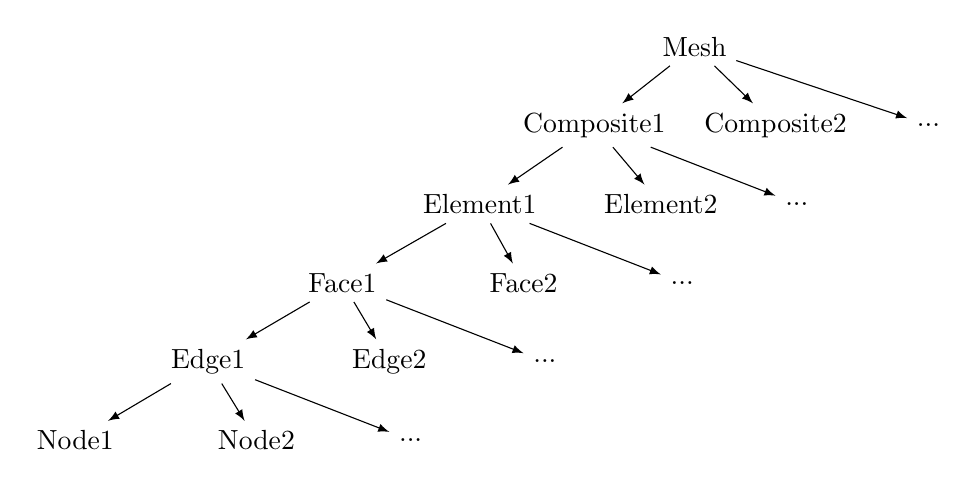
\begin{tikzpicture}[
  sibling distance=23mm, 
  level distance=10mm,
  edge from parent/.style={draw,-latex}, 
  grow=south,
  every node/.style={anchor=west}
]

% Root node
\node {Mesh}
  child {node {Composite1}
    child {node {Element1}
      child {node {Face1}
        child {node {Edge1}
          child {node {Node1}}
          child {node {Node2}}
          child {node {...}}}
        child {node {Edge2}}
        child {node {...}}}
      child {node {Face2}}
      child {node {...}}}
    child {node {Element2}}
    child {node {...}}}
  child {node {Composite2}}
  child [sibling distance=27mm]{node {...}};

\end{tikzpicture}
  \caption{}
  \label{fig:NekMesh_hierarchy}
\end{figure}

Meshes have a \textbf{dimensionality} of their own (eg. for a surface
mesh \texttt{expDim = 2}, for a volume mesh \texttt{expDim = 3}), and
exist in n-dimensional physical space (\texttt{physDim}, where
{\texttt{physDim} $\geq$ \texttt{expDim}). \textbf{Composites} are
  collections of elements. For elements which have the same
  dimensionality as the physical space they are in, they are grouped
  by their type. \textbf{Note:} boundary tri and quad elements are all
  grouped into a singular composite. \textbf{Boundary element} are
  elements that form the boundary of a mesh area/volume. These are one
  dimension lower than the physical dimension (eg. in 3D space, mesh
  volumes have boundary \textit{surfaces}).

\subsection{Vertex node ordering rules}
\label{sect:node_ordering}
\subsubsection{Collapsed points} 
NekMesh supports quadrilateral (quad) and triangular (tri) 2D
elements, and tetrahedral (tet), prism, pyramid (pyra) and hexahedral
(hex) 3D element. Elements with tri faces (all except quads and hexes)
use a collapsed coordinate systems (fig. \ref{fig:collapsed_coords})
\cite{textbook}, a feature which introduces constraints when
assembling and connecting 3D elements.

In the code, we indicate which node in a tri face is the collapsed point by giving it the highest node id (in \texttt{InputCGNS.cpp} and \texttt{InputStar.cpp} the node ordering is done in the function \texttt{ResetNodes}). Note that the relative ordering between nodes in \textit{different faces} (even if in the same element) has no affect.

\begin{figure}[h!]
    \centering
    \begin{subfigure}[b]{0.45\textwidth}
        \centering
        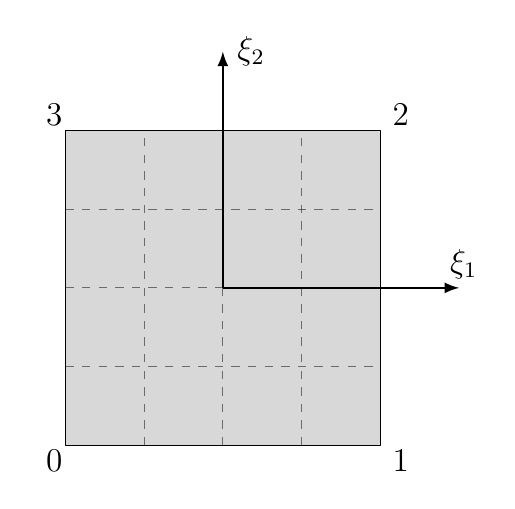
\begin{tikzpicture}[line join=bevel,scale=2,>=latex]
  \coordinate (n0) at (-1,-1);
  \coordinate (n1) at (1,-1);
  \coordinate (n2) at (1,1);
  \coordinate (n3) at (-1,1);

  \coordinate (n4) at (-0.5, -1);
  \coordinate (n5) at (0, -1);
  \coordinate (n6) at (0.5, -1);

  \coordinate (n7) at (1, -0.5);
  \coordinate (n8) at (1, 0);
  \coordinate (n9) at (1, 0.5);

  \coordinate (n10) at (0.5, 1);
  \coordinate (n11) at (0, 1);
  \coordinate (n12) at (-0.5, 1);

  \coordinate (n13) at (-1, 0.5);
  \coordinate (n14) at (-1, 0);
  \coordinate (n15) at (-1, -0.5);

  \coordinate (C) at (0, 0);
  \coordinate (j) at (0, 1.5);
  \coordinate (i) at (1.5, 0);

  \begin{scope}[blend mode=multiply]
    \fill[black!30,fill opacity=0.5] (n0) -- (n1) -- (n2) -- (n3) -- cycle;
  \end{scope}
  
  \draw (n0) -- (n1) -- (n2) -- (n3) -- cycle;
  \draw[dashed,opacity=0.5] (n4) -- (n12);
  \draw[dashed,opacity=0.5] (n5) -- (n11);
  \draw[dashed,opacity=0.5] (n6) -- (n10);
  \draw[dashed,opacity=0.5] (n15) -- (n7);
  \draw[dashed,opacity=0.5] (n14) -- (n8);
  \draw[dashed,opacity=0.5] (n13) -- (n9);

  \draw[thick, ->] (C) -- (i);
  \draw[thick, ->] (C) -- (j);
  \node at (1.5, 0.15) {\fontsize{12}{12} \selectfont $\xi_1$};
  \node at (0.15, 1.5) {\fontsize{12}{12} \selectfont $\xi_2$};
  \node at (-1.1, -1.1) {\fontsize{12}{12} \selectfont $0$};
  \node at (1.1, -1.1) {\fontsize{12}{12} \selectfont $1$};
  \node at (1.1, 1.1) {\fontsize{12}{12} \selectfont $2$};
  \node at (-1.1, 1.1) {\fontsize{12}{12} \selectfont $3$};

  
\end{tikzpicture}

        \caption{Coordinate system for the reference quadrilateral.}
        \label{fig:quad_coords}
    \end{subfigure}
    \hfill
    \begin{subfigure}[b]{0.45\textwidth}
        \centering
        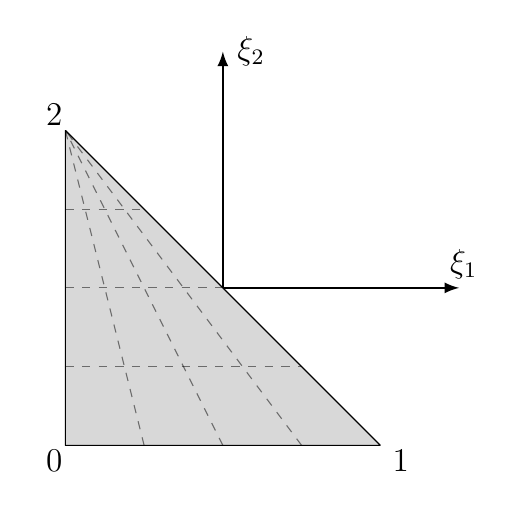
\begin{tikzpicture}[line join=bevel,scale=2,>=latex]
  \coordinate (n0) at (-1,-1);
  \coordinate (n1) at (1,-1);
  \coordinate (n2) at (-1,1);

  \coordinate (n3) at (-0.5, -1);
  \coordinate (n4) at (0, -1);
  \coordinate (n5) at (0.5, -1);

  \coordinate (n6) at (0.5, -0.5);
  \coordinate (n7) at (0, 0);
  \coordinate (n8) at (-0.5, 0.5);

  \coordinate (n9) at (-1, 0.5);
  \coordinate (n10) at (-1, 0);
  \coordinate (n11) at (-1, -0.5);

  \coordinate (C) at (0, 0);
  \coordinate (j) at (0, 1.5);
  \coordinate (i) at (1.5, 0);

  \begin{scope}[blend mode=multiply]
    \fill[black!30,fill opacity=0.5] (n0) -- (n1) -- (n2) -- cycle;
  \end{scope}
  
  \draw (n0) -- (n1) -- (n2) -- cycle;
  \draw[dashed,opacity=0.5] (n3) -- (n2);
  \draw[dashed,opacity=0.5] (n4) -- (n2);
  \draw[dashed,opacity=0.5] (n5) -- (n2);
  \draw[dashed,opacity=0.5] (n11) -- (n6);
  \draw[dashed,opacity=0.5] (n10) -- (n7);
  \draw[dashed,opacity=0.5] (n9) -- (n8);

  \draw[thick, ->] (C) -- (i);
  \draw[thick, ->] (C) -- (j);
  \node at (1.5, 0.15) {\fontsize{12}{12} \selectfont $\xi_1$};
  \node at (0.15, 1.5) {\fontsize{12}{12} \selectfont $\xi_2$};
  \node at (-1.1, -1.1) {\fontsize{12}{12} \selectfont $0$};
  \node at (1.1, -1.1) {\fontsize{12}{12} \selectfont $1$};
  \node at (-1.1, 1.1) {\fontsize{12}{12} \selectfont $2$};
  
\end{tikzpicture}

        \caption{Collapsed coordinate system for the reference triangle. Node 2 is considered the 'collapsed point'.}
        \label{fig:collapsed_coords}
    \end{subfigure}
    \caption{Coordinate systems for 2D elements/faces.}
    \label{fig:coords}
\end{figure}

\subsubsection{Tri interface rule}
This rule simply states that when tri faces on two elements meet, the collapsed point must be the same for each tri (fig. \ref{fig:tri_interface_rule}).

\begin{figure}[h!]
    \centering
    \begin{subfigure}[b]{0.45\textwidth}
        \centering
        \tdplotsetmaincoords{70}{60}

\begin{tikzpicture}[line join=bevel,tdplot_main_coords,scale=1.25,>=latex]

  \coordinate (a) at (-1, 1.5,-1);
  \coordinate (b) at ( 1, 1.5,-1);
  \coordinate (c) at ( 1, 3.5,-1);
  \coordinate (d) at (-1, 3.5,-1);
  \coordinate (e) at (-1, 1.5, 1);
  \coordinate (f) at (-1, 3.5, 1);
  
  \coordinate (ab1) at (-0.33, 1.5, -1);
  \coordinate (ab2) at (0.33, 1.5, -1);
  \coordinate (ae1) at (-1, 1.5, -0.33);
  \coordinate (ae2) at (-1, 1.5, 0.33);
  \coordinate (be1) at ( 0.33, 1.5, -0.33);
  \coordinate (be2) at (-0.33, 1.5, 0.33);
  
  \coordinate (dc1) at (-0.33, 3.5, -1);
  \coordinate (dc2) at (0.33, 3.5, -1);
  \coordinate (df1) at (-1, 3.5, -0.33);
  \coordinate (df2) at (-1, 3.5, 0.33);
  \coordinate (cf1) at (0.33, 3.5, -0.33);
  \coordinate (cf2) at (-0.33, 3.5, 0.33);
  
  \begin{scope}[blend mode=multiply]
    \fill[green!30,fill opacity=0.3] (a) -- (b) -- (e) -- cycle;
    \fill[black!30,fill opacity=0.3] (d) -- (c) -- (f) -- cycle;
  \end{scope}
  
  \draw(e) -- (b) -- (a) -- cycle;
  \draw (b) -- (c) -- (f) -- (e);
  \draw[dashed,opacity=0.5] (c) -- (d) -- (a);
  \draw[dashed,opacity=0.5] (d) -- (f);
  
  \draw [green!100](ab1) -- (e);
  \draw [green!100](ab2) -- (e);
  \draw [green!100](ae1) -- (be1);
  \draw [green!100](ae2) -- (be2);
  \draw [black!50](dc1) -- (f);
  \draw [black!50](dc2) -- (f);
  \draw [black!50](df1) -- (cf1);
  \draw [black!50](df2) -- (cf2);


  \coordinate (A) at (-1,-1,-1);
  \coordinate (B) at ( 1,-1,-1);
  \coordinate (C) at ( 1, 1,-1);
  \coordinate (D) at (-1, 1,-1);
  \coordinate (E) at (-1,-1, 1);
  \coordinate (F) at (-1, 1, 1);

  \coordinate (AB1) at (-0.33, -1, -1);
  \coordinate (AB2) at (0.33, -1, -1);
  \coordinate (AE1) at (-1,-1,-0.33);
  \coordinate (AE2) at (-1,-1,0.33);
  \coordinate (BE1) at ( 0.33,-1,-0.33);
  \coordinate (BE2) at ( -0.33,-1,0.33);

  \coordinate (DC1) at (-0.33, 1, -1);
  \coordinate (DC2) at (0.33, 1, -1);
  \coordinate (DF1) at (-1,1,-0.33);
  \coordinate (DF2) at (-1,1,0.33);
  \coordinate (CF1) at ( 0.33,1,-0.33);
  \coordinate (CF2) at ( -0.33,1,0.33);
  
  \begin{scope}[blend mode=multiply]
    \fill[black!30,fill opacity=0.3] (A) -- (B) -- (E) -- cycle;
    \fill[green!30,fill opacity=0.3] (D) -- (C) -- (F) -- cycle;
  \end{scope}
  
  \draw (A) -- (B) -- (E) -- cycle;
  \draw (B) -- (C) -- (F) -- (E);
  \draw[dashed,opacity=0.5] (C) -- (D) -- (A);
  \draw[dashed,opacity=0.5] (D) -- (F);

   \draw [black!50](AB1) -- (E);
   \draw [black!50](AB2) -- (E);
   \draw [black!50](AE1) -- (BE1);
   \draw [black!50](AE2) -- (BE2);
   \draw [green!100](DC1) -- (F);
   \draw [green!100](DC2) -- (F);
   \draw [green!100](DF1) -- (CF1);
   \draw [green!100](DF2) -- (CF2);
  

\end{tikzpicture}
        \caption{Valid element: neighbouring tri faces are alligned}
        \label{fig:prism_rule_ok_join}
    \end{subfigure}
    \hfill
    \begin{subfigure}[b]{0.45\textwidth}
        \centering
        \tdplotsetmaincoords{70}{60}

\begin{tikzpicture}[line join=bevel,tdplot_main_coords,scale=1.25,>=latex]

  \coordinate (a) at (-1, 1.5,-1);
  \coordinate (b) at ( 1, 1.5,-1);
  \coordinate (c) at ( 1, 3.5,-1);
  \coordinate (d) at (-1, 3.5,-1);
  \coordinate (e) at (-1, 1.5, 1);
  \coordinate (f) at (-1, 3.5, 1);
  
  \coordinate (ab1) at (-0.33, 1.5, -1);
  \coordinate (ab2) at (0.33, 1.5, -1);
  \coordinate (ae1) at (-1, 1.5, -0.33);
  \coordinate (ae2) at (-1, 1.5, 0.33);
  \coordinate (be1) at ( 0.33, 1.5, -0.33);
  \coordinate (be2) at (-0.33, 1.5, 0.33);
  
  \coordinate (dc1) at (-0.33, 3.5, -1);
  \coordinate (dc2) at (0.33, 3.5, -1);
  \coordinate (df1) at (-1, 3.5, -0.33);
  \coordinate (df2) at (-1, 3.5, 0.33);
  \coordinate (cf1) at (0.33, 3.5, -0.33);
  \coordinate (cf2) at (-0.33, 3.5, 0.33);
  
  \begin{scope}[blend mode=multiply]
    \fill[red!30,fill opacity=0.3] (a) -- (b) -- (e) -- cycle;
    \fill[black!30,fill opacity=0.3] (d) -- (c) -- (f) -- cycle;
  \end{scope}
  
  \draw(e) -- (b) -- (a) -- cycle;
  \draw (b) -- (c) -- (f) -- (e);
  \draw[dashed,opacity=0.5] (c) -- (d) -- (a);
  \draw[dashed,opacity=0.5] (d) -- (f);
  
  \draw [red!100](ab1) -- (be2);
  \draw [red!100](ab2) -- (be1);
  \draw [red!100](ae1) -- (b);
  \draw [red!100](ae2) -- (b);
  \draw [black!50](dc1) -- (cf2);
  \draw [black!50](dc2) -- (cf1);
  \draw [black!50](df1) -- (c);
  \draw [black!50](df2) -- (c);


  \coordinate (A) at (-1,-1,-1);
  \coordinate (B) at ( 1,-1,-1);
  \coordinate (C) at ( 1, 1,-1);
  \coordinate (D) at (-1, 1,-1);
  \coordinate (E) at (-1,-1, 1);
  \coordinate (F) at (-1, 1, 1);

  \coordinate (AB1) at (-0.33, -1, -1);
  \coordinate (AB2) at (0.33, -1, -1);
  \coordinate (AE1) at (-1,-1,-0.33);
  \coordinate (AE2) at (-1,-1,0.33);
  \coordinate (BE1) at ( 0.33,-1,-0.33);
  \coordinate (BE2) at ( -0.33,-1,0.33);

  \coordinate (DC1) at (-0.33, 1, -1);
  \coordinate (DC2) at (0.33, 1, -1);
  \coordinate (DF1) at (-1,1,-0.33);
  \coordinate (DF2) at (-1,1,0.33);
  \coordinate (CF1) at ( 0.33,1,-0.33);
  \coordinate (CF2) at ( -0.33,1,0.33);
  
  \begin{scope}[blend mode=multiply]
    \fill[black!30,fill opacity=0.3] (A) -- (B) -- (E) -- cycle;
    \fill[red!30,fill opacity=0.3] (D) -- (C) -- (F) -- cycle;
  \end{scope}
  
  \draw (A) -- (B) -- (E) -- cycle;
  \draw (B) -- (C) -- (F) -- (E);
  \draw[dashed,opacity=0.5] (C) -- (D) -- (A);
  \draw[dashed,opacity=0.5] (D) -- (F);

   \draw [black!50](AB1) -- (E);
   \draw [black!50](AB2) -- (E);
   \draw [black!50](AE1) -- (BE1);
   \draw [black!50](AE2) -- (BE2);
   \draw [red!100](DC1) -- (F);
   \draw [red!100](DC2) -- (F);
   \draw [red!100](DF1) -- (CF1);
   \draw [red!100](DF2) -- (CF2);
  

\end{tikzpicture}
        \caption{Invalid element: neighbouring tri faces are misalligned}
        \label{fig:prism_rule_bad_join}
    \end{subfigure}
    \caption{Tri interface rule}
    \label{fig:tri_interface_rule}
\end{figure}

\subsubsection{Prism rule}
For prism elements, the collapsed point on both the tri faces must correspond (ie. there must be an edge joining them) (fig. \ref{fig:prism_rule}). Combining this with rule 1., we see that in a prism line (line of prisms joined by their tri faces), they all must be oriented in the same way.

\begin{figure}[h!]
    \centering
    \begin{subfigure}[b]{0.45\textwidth}
        \centering
        \tdplotsetmaincoords{70}{50}

\begin{tikzpicture}[line join=bevel,tdplot_main_coords,scale=2,>=latex]
  \coordinate (A) at (-1,-1,-1);
  \coordinate (B) at ( 1,-1,-1);
  \coordinate (C) at ( 1, 1,-1);
  \coordinate (D) at (-1, 1,-1);
  \coordinate (E) at (-1,-1, 1);
  \coordinate (F) at (-1, 1, 1);

  \coordinate (AB1) at (-0.33, -1, -1);
  \coordinate (AB2) at (0.33, -1, -1);
  \coordinate (AE1) at (-1,-1,-0.33);
  \coordinate (AE2) at (-1,-1,0.33);
  \coordinate (BE1) at ( 0.33,-1,-0.33);
  \coordinate (BE2) at ( -0.33,-1,0.33);

  \coordinate (DC1) at (-0.33, 1, -1);
  \coordinate (DC2) at (0.33, 1, -1);
  \coordinate (DF1) at (-1,1,-0.33);
  \coordinate (DF2) at (-1,1,0.33);
  \coordinate (CF1) at ( 0.33,1,-0.33);
  \coordinate (CF2) at ( -0.33,1,0.33);
  
  \begin{scope}[blend mode=multiply]
    %\fill[black!30,fill opacity=0.5] (B) -- (C) -- (F) -- (E) -- cycle;
    \fill[green!30,fill opacity=0.3] (A) -- (B) -- (E) -- cycle;
    %\fill[black!50,fill opacity=0.5] (A) -- (B) -- (C) -- (D) -- cycle;
    \fill[green!30,fill opacity=0.3] (D) -- (C) -- (F) -- cycle;
    %\fill[black!70,fill opacity=0.5] (A) -- (D) -- (F) -- (E) -- cycle;
  \end{scope}
  
  \draw (A) -- (B) -- (E) -- cycle;
  \draw (B) -- (C) -- (F) -- (E);
  \draw[dashed,opacity=0.5] (C) -- (D) -- (A);
  \draw[dashed,opacity=0.5] (D) -- (F);

   \draw [green!100](AB1) -- (E);
   \draw [green!100](AB2) -- (E);
   \draw [green!100](AE1) -- (BE1);
   \draw [green!100](AE2) -- (BE2);
   \draw [green!100](DC1) -- (F);
   \draw [green!100](DC2) -- (F);
   \draw [green!100](DF1) -- (CF1);
   \draw [green!100](DF2) -- (CF2);
  
\end{tikzpicture}
        \caption{Valid element: two tri faces are alligned}
        \label{fig:prism_rule_ok}
    \end{subfigure}
    \hfill
    \begin{subfigure}[b]{0.45\textwidth}
        \centering
        \tdplotsetmaincoords{70}{50}

\begin{tikzpicture}[line join=bevel,tdplot_main_coords,scale=2,>=latex]
  \coordinate (A) at (-1,-1,-1);
  \coordinate (B) at ( 1,-1,-1);
  \coordinate (C) at ( 1, 1,-1);
  \coordinate (D) at (-1, 1,-1);
  \coordinate (E) at (-1,-1, 1);
  \coordinate (F) at (-1, 1, 1);

  \coordinate (AB1) at (-0.33, -1, -1);
  \coordinate (AB2) at (0.33, -1, -1);
  \coordinate (AE1) at (-1,-1,-0.33);
  \coordinate (AE2) at (-1,-1,0.33);
  \coordinate (BE1) at ( 0.33,-1,-0.33);
  \coordinate (BE2) at ( -0.33,-1,0.33);

  \coordinate (DC1) at (-0.33, 1, -1);
  \coordinate (DC2) at (0.33, 1, -1);
  \coordinate (DF1) at (-1,1,-0.33);
  \coordinate (DF2) at (-1,1,0.33);
  \coordinate (CF1) at ( 0.33,1,-0.33);
  \coordinate (CF2) at ( -0.33,1,0.33);
  
  \begin{scope}[blend mode=multiply]
    %\fill[black!30,fill opacity=0.5] (B) -- (C) -- (F) -- (E) -- cycle;
    \fill[red!30,fill opacity=0.3] (A) -- (B) -- (E) -- cycle;
    %\fill[black!50,fill opacity=0.5] (A) -- (B) -- (C) -- (D) -- cycle;
    \fill[red!30,fill opacity=0.3] (D) -- (C) -- (F) -- cycle;
    %\fill[black!70,fill opacity=0.5] (A) -- (D) -- (F) -- (E) -- cycle;
  \end{scope}
  
  \draw (A) -- (B) -- (E) -- cycle;
  \draw (B) -- (C) -- (F) -- (E);
  \draw[dashed,opacity=0.5] (C) -- (D) -- (A);
  \draw[dashed,opacity=0.5] (D) -- (F);

   \draw [red!100](AB1) -- (E);
   \draw [red!100](AB2) -- (E);
   \draw [red!100](AE1) -- (BE1);
   \draw [red!100](AE2) -- (BE2);

   \draw [red!100](DC1) -- (CF2);
   \draw [red!100](DC2) -- (CF1);
   \draw [red!100](DF1) -- (C);
   \draw [red!100](DF2) -- (C);
  
\end{tikzpicture}
        \caption{Invalid element: two tri faces are misalligned}
        \label{fig:prism_rule_bad}
    \end{subfigure}
    \caption{Prism rule}
    \label{fig:prism_rule}
\end{figure}


\subsubsection{Pyramid rule}
In a pyramid element, the collapsed point on all four tri faces must be at the apex of the pyramid (fig. \ref{fig:pyra_rule}).


\begin{figure}[h!]
    \centering
    \begin{subfigure}[b]{0.45\textwidth}
        \centering
        \tdplotsetmaincoords{70}{20}

\begin{tikzpicture}[line join=bevel,tdplot_main_coords,scale=2,>=latex]
  \coordinate (A) at (-1,-1,-1);
  \coordinate (B) at ( 1,-1,-1);
  \coordinate (C) at ( 1, 1,-1);
  \coordinate (D) at (-1, 1,-1);
  \coordinate (E) at (0, 0, 1);

  \coordinate (AB1) at (-0.33, -1, -1);
  \coordinate (AB2) at (0.33, -1, -1);
  \coordinate (AE1) at (-0.67,-0.67, -0.33);
  \coordinate (AE2) at (-0.33,-0.33, 0.33);
  \coordinate (BE1) at (0.67,-0.67, -0.33);
  \coordinate (BE2) at (0.33,-0.33, 0.33);

  \coordinate (BC1) at (1, -0.33, -1);
  \coordinate (BC2) at (1, 0.33, -1);
  \coordinate (CE1) at ( 0.67, 0.67, -0.33);
  \coordinate (CE2) at ( 0.33, 0.33, 0.33);
  
  \begin{scope}[blend mode=multiply]
    \fill[green!30,fill opacity=0.3] (A) -- (B) -- (E) -- cycle;
    \fill[green!30,fill opacity=0.3] (B) -- (C) -- (E) -- cycle;
  \end{scope}
  
  \draw (A) -- (B) -- (E) -- cycle;
  \draw (B) -- (C) -- (E) -- cycle;
  \draw[dashed,opacity=0.5] (C) -- (D) -- (A);
  \draw[dashed,opacity=0.5] (D) -- (E);

   \draw [green!100](AB1) -- (E);
   \draw [green!100](AB2) -- (E);
   \draw [green!100](AE1) -- (BE1);
   \draw [green!100](AE2) -- (BE2);

   \draw [green!100](BC1) -- (E);
   \draw [green!100](BC2) -- (E);
   \draw [green!100](BE1) -- (CE1);
   \draw [green!100](BE2) -- (CE2);
  
\end{tikzpicture}
        \caption{Valid element: collapsed points at the apex for all tri faces}
        \label{fig:pyra_rule_ok}
    \end{subfigure}
    \hfill
    \begin{subfigure}[b]{0.45\textwidth}
        \centering
        \tdplotsetmaincoords{70}{20}

\begin{tikzpicture}[line join=bevel,tdplot_main_coords,scale=2,>=latex]
  \coordinate (A) at (-1,-1,-1);
  \coordinate (B) at ( 1,-1,-1);
  \coordinate (C) at ( 1, 1,-1);
  \coordinate (D) at (-1, 1,-1);
  \coordinate (E) at (0, 0, 1);

  \coordinate (AB1) at (-0.33, -1, -1);
  \coordinate (AB2) at (0.33, -1, -1);
  \coordinate (AE1) at (-0.67,-0.67, -0.33);
  \coordinate (AE2) at (-0.33,-0.33, 0.33);
  \coordinate (BE1) at (0.67,-0.67, -0.33);
  \coordinate (BE2) at (0.33,-0.33, 0.33);

  \coordinate (BC1) at (1, -0.33, -1);
  \coordinate (BC2) at (1, 0.33, -1);
  \coordinate (CE1) at ( 0.67, 0.67, -0.33);
  \coordinate (CE2) at ( 0.33, 0.33, 0.33);
  
  \begin{scope}[blend mode=multiply]
    \fill[red!30,fill opacity=0.3] (A) -- (B) -- (E) -- cycle;
    \fill[red!30,fill opacity=0.3] (B) -- (C) -- (E) -- cycle;
  \end{scope}
  
  \draw (A) -- (B) -- (E) -- cycle;
  \draw (B) -- (C) -- (E) -- cycle;
  \draw[dashed,opacity=0.5] (C) -- (D) -- (A);
  \draw[dashed,opacity=0.5] (D) -- (E);

   \draw [red!100](AB1) -- (E);
   \draw [red!100](AB2) -- (E);
   \draw [red!100](AE1) -- (BE1);
   \draw [red!100](AE2) -- (BE2);

   \draw [red!100](BC1) -- (BE1);
   \draw [red!100](BC2) -- (BE2);
   \draw [red!100](CE1) -- (B);
   \draw [red!100](CE2) -- (B);
  
\end{tikzpicture}
        \caption{Invalid element: collapsed points not at the apex for all tri faces}
        \label{fig:pyra_rule_bad}
    \end{subfigure}
    \caption{Pyramid rule}
    \label{fig:pyra_rule}
\end{figure}

\subsubsection{Tet and Hex elements}
Tet and hex elements \ref{fig:hex_and_tet} are more flexible in their orientation due to their symmetry (and lack of tri faces in the case of hexes), so don't introduce any additional rules.

\begin{figure}[h!]
    \centering
    \begin{subfigure}[b]{0.45\textwidth}
        \centering
        \tdplotsetmaincoords{70}{60}

\begin{tikzpicture}[line join=bevel,tdplot_main_coords,scale=2.2,>=latex]
  \coordinate (A) at (-1,-1,-1);
  \coordinate (AB1) at (-0.33,-1,-1);
  \coordinate (AB2) at (0.33,-1,-1);
  \coordinate (AD1) at (-1,-1,-0.33);
  \coordinate (AD2) at (-1,-1,0.33);
  \coordinate (B) at ( 1,-1,-1);
  \coordinate (BC1) at ( 0.33,-0.33,-1);
  \coordinate (BC2) at ( -0.33,0.33,-1);
  \coordinate (BD1) at ( 0.33,-1,-0.33);
  \coordinate (BD2) at (-0.33,-1,0.33);
  \coordinate (C) at (-1, 1,-1);
  \coordinate (CD1) at (-1, 0.33,-0.33);
  \coordinate (CD2) at (-1, -0.33,0.33);
  \coordinate (D) at (-1,-1, 1);
  
  \begin{scope}[blend mode=multiply]
    \fill[green!30,fill opacity=0.3] (A) -- (B) -- (D) -- cycle;
    \fill[green!30,fill opacity=0.3] (B) -- (C) -- (D) -- cycle;
  \end{scope}

   \draw [green!100](AB1) -- (D);
   \draw [green!100](AB2) -- (D);
   \draw [green!100](BC1) -- (D);
   \draw [green!100](BC2) -- (D);
   \draw [green!100](AD1) -- (BD1) -- (CD1);
   \draw [green!100](AD2) -- (BD2) -- (CD2);

  \draw (A) -- (B) -- (D) -- cycle;
  \draw (B) -- (C) -- (D);
  \draw[dashed,opacity=0.5] (A) -- (C);

\end{tikzpicture}

        \caption{}
        \label{fig:tet_ok}
    \end{subfigure}
    \hfill
    \begin{subfigure}[b]{0.45\textwidth}
        \centering
        \tdplotsetmaincoords{70}{50}

\begin{tikzpicture}[line join=bevel,tdplot_main_coords,scale=2,>=latex]
  \coordinate (A) at (-1,-1,-1);
  \coordinate (AB1) at (-0.33,-1,-1);
  \coordinate (AB2) at (0.33,-1,-1);
  \coordinate (AE1) at (-1,-1,-0.33);
  \coordinate (AE2) at (-1,-1,0.33);
  \coordinate (B) at ( 1,-1,-1);
  \coordinate (BC1) at ( 1,-0.33,-1);
  \coordinate (BC2) at ( 1,0.33,-1);
  \coordinate (BF1) at (1,-1,-0.33);
  \coordinate (BF2) at (1,-1,0.33);
  \coordinate (C) at ( 1, 1,-1);
  \coordinate (CG1) at (1,1,-0.33);
  \coordinate (CG2) at (1,1,0.33);
  \coordinate (D) at (-1, 1,-1);
  \coordinate (E) at (-1,-1, 1);
  \coordinate (EF1) at (-0.33,-1,1);
  \coordinate (EF2) at (0.33,-1,1);
  \coordinate (EH1) at (-1,-0.33, 1);
  \coordinate (EH2) at (-1,0.33, 1);
  \coordinate (F) at ( 1,-1, 1);
  \coordinate (FG1) at ( 1,-0.33,1);
  \coordinate (FG2) at ( 1,0.33,1);
  \coordinate (G) at ( 1, 1, 1);
  \coordinate (GH1) at ( 0.33, 1, 1);
  \coordinate (GH2) at (-0.33, 1, 1);
  \coordinate (H) at (-1, 1, 1);
  
  \begin{scope}[blend mode=multiply]
    \fill[green!30,fill opacity=0.3] (A) -- (B) -- (F) -- (E) -- cycle;
    \fill[green!30,fill opacity=0.3] (B) -- (C) -- (G) -- (F) -- cycle;
    \fill[green!30,fill opacity=0.3] (E) -- (F) -- (G) -- (H) -- cycle;
  \end{scope}

   \draw [green!100](AB1) -- (EF1) -- (GH2);
   \draw [green!100](AB2) -- (EF2) -- (GH1);
   \draw [green!100](BC1) -- (FG1) -- (EH1);
   \draw [green!100](BC2) -- (FG2) -- (EH2);
   \draw [green!100](AE1) -- (BF1) -- (CG1);
   \draw [green!100](AE2) -- (BF2) -- (CG2);
  
  \draw (A) -- (B) -- (C);
  \draw (A) -- (E);
  \draw (B) -- (F);
  \draw (C) -- (G);
  \draw (E) -- (F) -- (G) -- (H) -- cycle;

  \draw[dashed,opacity=0.5] (D) -- (H);
  \draw[dashed,opacity=0.5] (C) -- (D) -- (A);

\end{tikzpicture}
        \caption{}
        \label{fig:hex_ok}
    \end{subfigure}
    \caption{Hex and tet elements...}
    \label{fig:hex_and_tet}
\end{figure}

\subsubsection{Impossible meshes}
When we combine the three rules simultaniously, there are a few mesh cases which are impossible to mesh \ref{fig:pyra_impossible}, but it is considered the responsibility of the mesh generator to avoid these. Therefore NekMesh deals with meshes that \textit{are} possible \textit{and} are likely to be produced my a CFD mesh generator.\\

\begin{figure}[h!]
  \centering
  \tdplotsetmaincoords{70}{15}

\begin{tikzpicture}[line join=bevel,tdplot_main_coords,scale=2,>=latex]
  \coordinate (A) at (-1,-1,-1);
  \coordinate (B) at ( 1,-1,-1);
  \coordinate (C) at ( 1, 1,-1);
  \coordinate (D) at (-1, 1,-1);
  \coordinate (E) at (0, 0, 1);

  \coordinate (BE1) at (0.67,-0.67, -0.33);
  \coordinate (BE2) at (0.33,-0.33, 0.33);
  \coordinate (BC1) at (1, -0.33, -1);
  \coordinate (BC2) at (1, 0.33, -1);
  \coordinate (CE1) at ( 0.67, 0.67, -0.33);
  \coordinate (CE2) at ( 0.33, 0.33, 0.33);
  
  \begin{scope}[blend mode=multiply]
    \fill[red!30,fill opacity=0.3] (B) -- (C) -- (E) -- cycle;
  \end{scope}
  
   \draw [red!100](BC1) -- (E);
   \draw [red!100](BC2) -- (E);
   \draw [red!100](BE1) -- (CE1);
   \draw [red!100](BE2) -- (CE2);

  \draw (A) -- (B) -- (E) -- cycle;
  \draw (B) -- (C) -- (E) -- cycle;
  \draw[dashed,opacity=0.5] (C) -- (D) -- (A);
  \draw[dashed,opacity=0.5] (D) -- (E);

  % ---------------------------------------------------------------------

  \coordinate (a) at (0.5, 0, 1);
  \coordinate (b) at (1.5, 1, -1);
  \coordinate (c) at (3.5, 1, 0);
  \coordinate (d) at (2.5, 0, 2);
  \coordinate (e) at (1.5, -1, -1);
  
  \coordinate (ab1) at (0.83, 0.33, 0.33);
  \coordinate (ab2) at (1.17, 0.67, -0.33);
  \coordinate (ae1) at (1.17, -0.67, -0.33);
  \coordinate (ae2) at (0.83, -0.33, 0.33);
  \coordinate (be1) at (1.5, 0.33, -1);
  \coordinate (be2) at (1.5, -0.33, -1);
  
  \begin{scope}[blend mode=multiply]
      \fill[red!30,fill opacity=0.3] (a) -- (b) -- (e) -- cycle;
  \end{scope}
  
  \draw [red!100](ab1) -- (e);
  \draw [red!100](ab2) -- (e);
  \draw [red!100](ae1) -- (be2);
  \draw [red!100](ae2) -- (be1);
  
  \draw[dashed,opacity=0.5] (c) -- (b) -- (a);
  \draw[dashed,opacity=0.5] (b) -- (e);
  \draw (a) -- (e);
  \draw (c) -- (d) -- (a);
  \draw (c) -- (e) -- (d);
  
\end{tikzpicture}
  \caption{}
  \label{fig:pyra_impossible}
\end{figure}

Since pyramid elements are the cause of these impossible meshes, one method used to rectify problematic pyramids is to use \textit{pyramid shielding} (fig. \ref{fig:pyramid_shielding}). The idea is to replace any problematic pyramid with a smaller pyramid, plus four tets \textit{shielding} the triangular pyramid faces from any neighbouring pyramid or prism elements. This decouples the pyramid's apex from neighbouring elements, due to the aforementioned flexibility of tets.

\begin{figure}[h!]
    \centering
    \begin{subfigure}[b]{0.45\textwidth}
        \centering
        \tdplotsetmaincoords{70}{30}

\begin{tikzpicture}[line join=bevel,tdplot_main_coords,scale=2,>=latex]
  \coordinate (A) at (-1,-1,-1);
  \coordinate (B) at ( 1,-1,-1);
  \coordinate (C) at ( 1, 1,-1);
  \coordinate (D) at (-1, 1,-1);
  \coordinate (E) at (0, 0, 1);
  
  \begin{scope}[blend mode=multiply]
    \fill[black!30,fill opacity=0.3] (A) -- (B) -- (E) -- cycle;
    \fill[black!30,fill opacity=0.3] (C) -- (D) -- (E) -- cycle;
    \fill[black!30,fill opacity=0.3] (A) -- (B) -- (C) -- (D) -- cycle;
    \fill[black!30,fill opacity=0.3] (A) -- (D) -- (E) -- cycle;
    \fill[black!30,fill opacity=0.3] (B) -- (C) -- (E) -- cycle;
  \end{scope}
  
  \draw[dashed,opacity=0.5] (A) -- (B) -- (E) -- cycle;
  \draw[dashed,opacity=0.5] (B) -- (C) -- (E) -- cycle;
  \draw[dashed,opacity=0.12] (C) -- (D) -- (A);
  \draw[dashed,opacity=0.12] (D) -- (E);
  
\end{tikzpicture}
        \caption{Before}
        \label{fig:pyramid_shielding-before}
    \end{subfigure}
    \hfill
    \begin{subfigure}[b]{0.45\textwidth}
        \centering
        \raisebox{-5mm}{ % Adjust this value to move the second subfigure down
            \tdplotsetmaincoords{70}{30}

\begin{tikzpicture}[line join=bevel,tdplot_main_coords,scale=2,>=latex]
  \coordinate (A) at (-1,-1,-1);
  \coordinate (B) at ( 1,-1,-1);
  \coordinate (C) at ( 1, 1,-1);
  \coordinate (D) at (-1, 1,-1);
  \coordinate (F) at ( 0, 0, 0);
  
  \coordinate (A1) at (-1,-1.2,-0.8);
  \coordinate (B1) at ( 1,-1.2,-0.8);
  \coordinate (E1) at ( 0,-0.2, 1.2);
  \coordinate (F1) at ( 0,-0.2, 0.2);
  
  \coordinate (B2) at ( 1.2,-1,-0.8);
  \coordinate (C2) at ( 1.2, 1,-0.8);
  \coordinate (E2) at ( 0.2, 0, 1.2);
  \coordinate (F2) at ( 0.2, 0, 0.2);
  
  \coordinate (C3) at ( 1, 1.2,-0.8);
  \coordinate (D3) at (-1, 1.2,-0.8);
  \coordinate (E3) at ( 0, 0.2, 1.2);
  \coordinate (F3) at ( 0, 0.2, 0.2);
  
  \coordinate (A4) at (-1.2,-1,-0.8);
  \coordinate (D4) at (-1.2, 1,-0.8);
  \coordinate (E4) at (-0.2, 0, 1.2);
  \coordinate (F4) at (-0.2, 0, 0.2);

  %-----------------------------------------------------------------
  
  \draw[magenta] (C3) -- (D3) -- (E3) -- cycle;
  \draw[magenta] (C3) -- (F3) -- (E3);
  \draw[magenta] (D3) -- (F3);
  
  \begin{scope}
    \fill[magenta!30,fill opacity=0.5] (C3) -- (D3) -- (E3) -- cycle;
    \fill[magenta!30,fill opacity=0.5] (C3) -- (D3) -- (F3) -- cycle;
    \fill[magenta!30,fill opacity=0.5] (C3) -- (E3) -- (F3) -- cycle;
    \fill[magenta!30,fill opacity=0.5] (D3) -- (E3) -- (F3) -- cycle;
  \end{scope}
  
  \draw[yellow] (D4) -- (A4) -- (E4) -- cycle;
  \draw[yellow] (D4) -- (F4) -- (E4);
  \draw[yellow,opacity=0.2] (A4) -- (F4);
  
  \begin{scope}
    \fill[yellow!30,fill opacity=0.5] (D4) -- (A4) -- (E4) -- cycle;
    \fill[yellow!30,fill opacity=0.5] (D4) -- (A4) -- (F4) -- cycle;
    \fill[yellow!30,fill opacity=0.5] (D4) -- (E4) -- (F4) -- cycle;
    \fill[yellow!30,fill opacity=0.5] (A4) -- (E4) -- (F4) -- cycle;
  \end{scope}
  
  \draw (A) -- (B) -- (F) -- cycle;
  \draw (B) -- (C) -- (F) -- cycle;
  \draw[opacity=0.2] (C) -- (D) -- (A);
  \draw[opacity=0.2] (D) -- (F);

  \begin{scope}[blend mode=multiply]
    \fill[black!30,fill opacity=0.5] (A) -- (B) -- (F) -- cycle;
    \fill[black!30,fill opacity=0.5] (C) -- (D) -- (F) -- cycle;
    \fill[black!30,fill opacity=0.5] (A) -- (B) -- (C) -- (D) -- cycle;
    \fill[black!30,fill opacity=0.5] (A) -- (D) -- (F) -- cycle;
    \fill[black!30,fill opacity=0.5] (B) -- (C) -- (F) -- cycle;
  \end{scope}

  \draw[orange] (B2) -- (C2) -- (E2) -- cycle;
  \draw[orange] (B2) -- (F2) -- (E2);
  \draw[orange,opacity=0.2] (C2) -- (F2);
  
  \begin{scope}
    \fill[orange!30,fill opacity=0.5] (B2) -- (C2) -- (E2) -- cycle;
    \fill[orange!30,fill opacity=0.5] (B2) -- (C2) -- (F2) -- cycle;
    \fill[orange!30,fill opacity=0.5] (B2) -- (E2) -- (F2) -- cycle;
    \fill[orange!30,fill opacity=0.5] (C2) -- (E2) -- (F2) -- cycle;
  \end{scope}

  \draw[blue] (A1) -- (B1) -- (E1) -- cycle;
  \draw[blue,opacity=0.2] (A1) -- (F1) -- (E1);
  \draw[blue,opacity=0.2] (B1) -- (F1);
  
    \begin{scope}
      \fill[blue!30,fill opacity=0.5] (A1) -- (B1) -- (E1) -- cycle;
      \fill[blue!30,fill opacity=0.5] (A1) -- (B1) -- (F1) -- cycle;
      \fill[blue!30,fill opacity=0.5] (A1) -- (E1) -- (F1) -- cycle;
      \fill[blue!30,fill opacity=0.5] (B1) -- (E1) -- (F1) -- cycle;
    \end{scope}
  
\end{tikzpicture}
        }
        \caption{After}
        \label{fig:pyramid_shielding-after}
    \end{subfigure}
    \caption{Before and after of the process of pyramid shielding. The pyra no longer restricts the orientation of neighbouring elements, so the impossible cases are avoided.}
    \label{fig:pyramid_shielding}
\end{figure}

\subsubsection{Implementation}
Assuming we are given a valid mesh, we now need an algorithm (see alg. \ref{alg:ResetNodes}) to order the nodes to define the orientation of the elements in accordance with the three rules. In \texttt{InputCGNS.cpp} and \texttt{InputStar.cpp}, this is implemented as the function \texttt{ResetNodes}.\\

\SetKwComment{Comment}{/* }{}
\begin{algorithm}[hbt!]
\caption{Setting ordering of node IDs in mesh}
\label{alg:ResetNodes}
    nodeID $\gets 0$ \Comment*[r]{stores the lowest available ID}
revNodeID $\gets$ numNodes $ - 1$ \Comment*[r]{stores the highest available ID}

\Comment{assign the apex node as the collapsed point and set the orientation of any prism lines that are connected to a pyramid tri face}
\ForEach{pyramid : pyramids}{
    \Comment{give the apex node the highest available ID}
    \textit{apex node} $\gets$ revNodeID\;
    revNodeID $\gets$ revNodeID - 1\;
    
    \ForEach{tri : pyramid tri faces}{
        \If{tri is shared with another pyramid}{
            \textbf{assert:} \textit{other pyramid shares the same apex node}\;
        }\ElseIf{tri is shared with a prism}{
            \textit{define the prism line}\;
            \Comment{traverse the prism line, recursively assigning the highest available ID to the corresponding node}
        }\Else{
            \Comment{it is either shared with a tet or ends in free space}
            continue\;
        }
    }
}

\Comment{set the orientation of the remaining prisms}
\ForEach{prism : prisms}{
    \If{any nodes have ID}{
        \Comment{this prism has already been dealt with}
        continue\;
    }
    \textit{create a list of the prisms in the prism line}\;
    \textit{define the prism line}\;
}

\Comment{give the remaining nodes an ID (low to high)}
\ForEach{node : nodes}{
    \If{node has ID}{
        continue\;
    }
    \Comment{Give node the lowest available ID}
    \textit{node} $\gets$ nodeID\;
    nodeID $\gets$ nodeID + 1\;
}
\end{algorithm}

Let's work through a simple example implementation. Say we are given the test mesh in fig \ref{fig:ResetNodes_example}; it contains 6 elements (2 pyras and 4 prisms) and 14 nodes. We must assign each of the nodes a unique ID (0-13), compatible with the three rules.

\begin{enumerate}
  \item{Label the apex of the first pyra (0) with the highest available ID (13).}
  \item{Pyra 0 shares a tri face with prism 2, so we must ID the corresponding node (12) on the opposite face of prism 2.}
  \item{We move to the next pyra (1) and assert that of all the ID'd nodes, the apex has the highest ID (true, since only the apex has been ID'd).}
  \item{With the pyramids correctly oriented, we move to the \textit{untouched} prisms (3, 4, 5), which all form a prism line. We arbitrarily assign the line of nodes labelled 11-8-5-2 as \textit{the} line of collapsed points and ensure that the points along this line have the highest ID on their respective tri faces.}
  \item{We have now labelled all the nodes, but if any were yet unlabelled, we would give them the remaining IDs (from low to high).}
\end{enumerate}

\begin{figure}[h!]
  \centering
  \newcommand{\nodeLabel}[3]{
    \node[color=#3, fill=white, opacity=0.9] at (#1) {\fontsize{14}{14}\selectfont #2}
}

\tdplotsetmaincoords{70}{20}
\begin{tikzpicture}[line join=bevel,tdplot_main_coords,scale=2,>=latex]
  \coordinate (A) at (-1,-1,-1);
  \coordinate (B) at ( 1,-1,-1);
  \coordinate (C) at ( 1, 1,-1);
  \coordinate (D) at (-1, 1,-1);
  \coordinate (E) at (0, 0, 1);
  
  \coordinate (A') at (2,-1,-1);
  \coordinate (B') at (4,-1,-1);
  \coordinate (C') at (4, 1,-1);
  \coordinate (D') at (2, 1,-1);
  \coordinate (E') at (3, 0, 1);

  \coordinate (U) at (-1,0,-2.5);
  \coordinate (V) at (1,0,-2.5);
  \coordinate (W) at (2,0,-2.5);
  \coordinate (X) at (4,0,-2.5);
  
  \coordinate (el0) at (0,   0, -0.2);  % pyr 
  \coordinate (el1) at (3,   0, -0.2);  % pyr
  \coordinate (el2) at (1.5, 0, -0.2);  % pris
  \coordinate (el3) at (0,   0, -1.75); % pris 
  \coordinate (el4) at (3,   0, -1.75); % pris
  \coordinate (el5) at (1.5, 0, -1.75); % pris
  
  \draw (A) -- (B) -- (E) -- cycle;
  \draw[dashed,opacity=0.5] (B) -- (C) -- (E) -- cycle;
  \draw[dashed,opacity=0.5] (C) -- (D) -- (A);
  \draw[dashed,opacity=0.5] (D) -- (E);
  
  \draw (B) -- (A');
  \draw[dashed,opacity=0.5] (C) -- (D');
  \draw (E) -- (E');

  \draw (A') -- (B') -- (E') -- cycle;
  \draw (B') -- (C') -- (E') -- cycle;
  \draw[dashed,opacity=0.5] (C') -- (D') -- (A');
  \draw[dashed,opacity=0.5] (D') -- (E');

  \draw (A) -- (U) -- (V) -- (B);
  \draw (A') -- (W) -- (X) -- (B');
  \draw (V) -- (W);
  \draw (X) -- (C');
  \draw[dashed,opacity=0.5] (U) -- (D);
  \draw[dashed,opacity=0.5] (V) -- (C);
  \draw[dashed,opacity=0.5] (W) -- (D');

  \nodeLabel{E} {13} {red};
  \nodeLabel{E'}{12}{red};
  \nodeLabel{A} {10} {red};
  \nodeLabel{B} {7} {red};
  \nodeLabel{C} {6} {red};
  \nodeLabel{D} {9} {red};
  \nodeLabel{A'}{4}{red};
  \nodeLabel{B'}{1}{red};
  \nodeLabel{C'}{0}{red};
  \nodeLabel{D'}{3}{red};
  \nodeLabel{U} {11} {red};
  \nodeLabel{V} {8} {red};
  \nodeLabel{W} {5} {red};
  \nodeLabel{X} {2} {red};

  \nodeLabel{el0}{0}{blue};
  \nodeLabel{el1}{1}{blue};
  \nodeLabel{el2}{2}{blue};
  \nodeLabel{el3}{3}{blue};
  \nodeLabel{el4}{4}{blue};
  \nodeLabel{el5}{5}{blue};
  
  
\end{tikzpicture}
  \caption{Node ordering determined by \texttt{ResetNodes} algorithm. Element IDs (already given): blue, node IDs: red.}
  \label{fig:ResetNodes_example}
\end{figure}

\subsection{Higher-order node ordering rules}
\label{sect:HO_node_ordering}
As well as the order of the global node IDs, we also need to take care
with the ordering of higher order nodes when creating elements, since
the NekMesh convention is different from other formats (namely .gmsh
and .cgns). Shown in figure \ref{fig:ho_2D_elements}, we can see that
the method for ordering quad and tri nodes is the same: primary nodes
(in black) are always included (clockwise), followed by mid-edge nodes
(in red) for \textit{all} higher order elements (also
clockwise). Mid-face nodes (in blue) are optional, but if included
they are next (ordered row-by-row).

\begin{figure}[h!]
    \centering
    \begin{subfigure}[b]{0.45\textwidth}
        \centering
        \newcommand{\nodeLabel}[3]{
    \node[color=#3, fill=white, opacity=0.9] at (#1) {\fontsize{10}{10}\selectfont #2}
}

\newcommand{\drawQuad}[4]{
    \coordinate (midMid) at ($  ($(#1) !0.5! (#2)$)  !0.5!  ($(#3) !0.5! (#4)$)  $);%
    \coordinate (l0) at ($ (#1) !0.4! (midMid) $);%
    \coordinate (l1) at ($ (#2) !0.4! (midMid) $);%
    \coordinate (l2) at ($ (#3) !0.4! (midMid) $);%
    \coordinate (l3) at ($ (#4) !0.4! (midMid) $);%
    \coordinate (l4) at ($ (l3) !0.33! (l0) $);%
    \draw[->, color=blue, thick] (l0) -- (l1) -- (l2) -- (l3) -- (l4)
}

\newcommand{\drawQuadFace}[5]{
    \coordinate (midMid) at ($  ($(#1) !0.5! (#2)$)  !0.5!  ($(#3) !0.5! (#4)$)  $);%
    \coordinate (l0) at ($ (#1) !0.4! (midMid) $);%
    \coordinate (l1) at ($ (#2) !0.4! (midMid) $);%
    \coordinate (l2) at ($ (#3) !0.4! (midMid) $);%
    \coordinate (l3) at ($ (#4) !0.4! (midMid) $);%
    \coordinate (l4) at ($ (l3) !0.33! (l0) $);%
    \nodeLabel{midMid}{#5}{blue};%
    \draw[->, color=blue, thick] (l0) -- (l1) -- (l2) -- (l3) -- (l4)%
}

\newcommand{\drawOffsetArrow}[2]{%
  \draw[->, color=red, thick] 
    ($ (#1)!0.1!(#2) $)  -- ($ (#2)!0.1!(#1) $)
}

\begin{tikzpicture}[line join=bevel,scale=2,>=latex]
  \coordinate (n0) at (-1,-1);%
  \coordinate (n1) at (1,-1);%
  \coordinate (n2) at (1,1);%
  \coordinate (n3) at (-1,1);%

  \coordinate (l0) at (-0.75, -0.75);%
  \coordinate (l1) at (0.75, -0.75);%
  \coordinate (l2) at (0.75, 0.75);%
  \coordinate (l3) at (-0.75, 0.75);%
  \coordinate (l4) at (-0.75, 0.25);%
  
  
  % \draw[thick] (n0) -- (n1) -- (n2) -- (n3) -- cycle;%
  \drawOffsetArrow{n0}{n1};%
  \drawOffsetArrow{n1}{n2};%
  \drawOffsetArrow{n2}{n3};%
  \drawOffsetArrow{n3}{n0};%
  \drawQuad{n0}{n1}{n2}{n3};%

  \nodeLabel{n0}{0}{black};%
  \nodeLabel{n1}{1 }{black};%
  \nodeLabel{n2}{2 }{black};%
  \nodeLabel{n3}{3 }{black};%

\end{tikzpicture}

        \caption{Orientation of quad face is indicated by the arrow (0 $\rightarrow$ 1 $\rightarrow$ 2 $\rightarrow$ 3). This is same representation will be used for 3D elements.}
        \label{fig:ho_quad-arrow}
    \end{subfigure}
    \hfill
    \begin{subfigure}[b]{0.45\textwidth}
        \centering
        \newcommand{\nodeLabel}[3]{
    \node[color=#3, fill=white, opacity=0.9] at (#1) {\fontsize{10}{10}\selectfont #2}
}

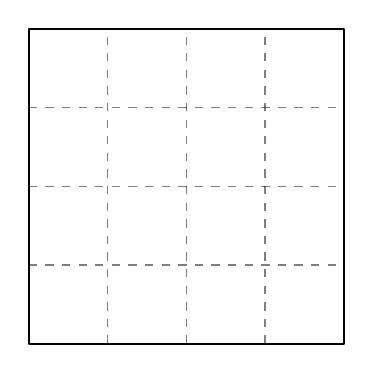
\begin{tikzpicture}[line join=bevel,scale=2,>=latex]
  \coordinate (n0) at (-1,-1);
  \coordinate (n1) at (1,-1);
  \coordinate (n2) at (1,1);
  \coordinate (n3) at (-1,1);

  \coordinate (n4) at (-0.5, -1);
  \coordinate (n5) at (0, -1);
  \coordinate (n6) at (0.5, -1);

  \coordinate (n7) at (1, -0.5);
  \coordinate (n8) at (1, 0);
  \coordinate (n9) at (1, 0.5);

  \coordinate (n10) at (0.5, 1);
  \coordinate (n11) at (0, 1);
  \coordinate (n12) at (-0.5, 1);

  \coordinate (n13) at (-1, 0.5);
  \coordinate (n14) at (-1, 0);
  \coordinate (n15) at (-1, -0.5);

  \coordinate (n16) at (-0.5, -0.5);
  \coordinate (n17) at (0, -0.5);
  \coordinate (n18) at (0.5, -0.5);

  \coordinate (n19) at (-0.5, 0);
  \coordinate (n20) at (0, 0);
  \coordinate (n21) at (0.5, 0);

  \coordinate (n22) at (-0.5, 0.5);
  \coordinate (n23) at (0, 0.5);
  \coordinate (n24) at (0.5, 0.5);
  
  
  \draw[thick] (n0) -- (n1) -- (n2) -- (n3) -- cycle;
  \draw[dashed,opacity=0.5] (n4) -- (n12);
  \draw[dashed,opacity=0.5] (n5) -- (n11);
  \draw[dashed,opacity=0.5] (n6) -- (n10);
  \draw[dashed,opacity=0.5] (n15) -- (n7);
  \draw[dashed,opacity=0.5] (n14) -- (n8);
  \draw[dashed,opacity=0.5] (n13) -- (n9);

  \nodeLabel{n0}{0}{black};
  \nodeLabel{n1}{1 }{black};
  \nodeLabel{n2}{2 }{black};
  \nodeLabel{n3}{3 }{black};
  \nodeLabel{n4}{4 }{red};
  \nodeLabel{n5}{5 }{red};
  \nodeLabel{n6}{6 }{red};
  \nodeLabel{n7}{7 }{red};
  \nodeLabel{n8}{8 }{red};
  \nodeLabel{n9}{9 }{red};
  \nodeLabel{n10}{10}{red};
  \nodeLabel{n11}{11}{red};
  \nodeLabel{n12}{12}{red};
  \nodeLabel{n13}{13}{red};
  \nodeLabel{n14}{14}{red};
  \nodeLabel{n15}{15}{red};
  
  \nodeLabel{n16}{16}{blue};
  \nodeLabel{n17}{17}{blue};
  \nodeLabel{n18}{18}{blue};
  \nodeLabel{n19}{19}{blue};
  \nodeLabel{n20}{20}{blue};
  \nodeLabel{n21}{21}{blue};
  \nodeLabel{n22}{22}{blue};
  \nodeLabel{n23}{23}{blue};
  \nodeLabel{n24}{24}{blue};

\end{tikzpicture}
        \caption{Node ordering given for a 4th order quad element with mid-edge and mid-face nodes.}
        \label{fig:ho_quad-numbered}
    \end{subfigure}
    \begin{subfigure}[b]{0.45\textwidth}
        \centering
        \newcommand{\nodeLabel}[3]{
    \node[color=#3, fill=white, opacity=0.9] at (#1) {\fontsize{10}{10}\selectfont #2}
}

\newcommand{\drawOffsetArrow}[2]{%
  \draw[->, color=red, thick] 
    ($ (#1)!0.1!(#2) $)  -- ($ (#2)!0.1!(#1) $)
}

\newcommand{\drawTri}[3]{
    \coordinate (midMid) at ($  ($(#1) !0.5! (#2)$)  !0.33!  (#3)  $);
    \coordinate (l0) at ($ (#1) !0.4! (midMid) $);
    \coordinate (l1) at ($ (#2) !0.4! (midMid) $);
    \coordinate (l2) at ($ (#3) !0.4! (midMid) $);
    \coordinate (l3) at ($ (l2) !0.33! (l0) $);
    \draw[->, color=blue, thick] (l0) -- (l1) -- (l2) -- (l3)
}

\newcommand{\drawTriFace}[4]{
    \coordinate (midMid) at ($  ($(#1) !0.5! (#2)$)  !0.33!  (#3)  $);
    \coordinate (l0) at ($ (#1) !0.4! (midMid) $);
    \coordinate (l1) at ($ (#2) !0.4! (midMid) $);
    \coordinate (l2) at ($ (#3) !0.4! (midMid) $);
    \coordinate (l3) at ($ (l2) !0.33! (l0) $);
    \nodeLabel{midMid}{#4}{blue};
    \draw[->, color=blue, thick] (l0) -- (l1) -- (l2) -- (l3)
}


\begin{tikzpicture}[line join=bevel,scale=2,>=latex]
  \coordinate (n0) at (-1,-1);
  \coordinate (n1) at (1,-1);
  \coordinate (n2) at (-1,1);
  
  \coordinate (l0) at (-0.75, -0.75);
  \coordinate (l1) at (0.3, -0.75);
  \coordinate (l2) at (-0.75, 0.3);
  \coordinate (l3) at (-0.75, -0.2);
  
%  \draw[thick] (n0) -- (n1) -- (n2) -- cycle;
  \drawOffsetArrow{n0}{n1};
  \drawOffsetArrow{n1}{n2};
  \drawOffsetArrow{n2}{n0};
  \drawTri{n0}{n1}{n2};

  \nodeLabel{n0}{0 }{black};
  \nodeLabel{n1}{1 }{black};
  \nodeLabel{n2}{2 }{black};

\end{tikzpicture}

        \caption{Orientation of tri face is indicated by the arrow (0 $\rightarrow$ 1 $\rightarrow$ 2 $\rightarrow$ 3).}
        \label{fig:ho_tri-arrow}
    \end{subfigure}
    \hfill
    \begin{subfigure}[b]{0.45\textwidth}
        \centering
        \newcommand{\nodeLabel}[3]{
    \node[color=#3, fill=white, opacity=0.9] at (#1) {\fontsize{10}{10}\selectfont #2}
}

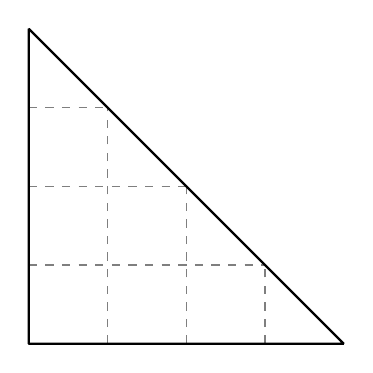
\begin{tikzpicture}[line join=bevel,scale=2,>=latex]
  \coordinate (n0) at (-1,-1);
  \coordinate (n1) at (1,-1);
  \coordinate (n2) at (-1,1);

  \coordinate (n3) at (-0.5, -1);
  \coordinate (n4) at (0, -1);
  \coordinate (n5) at (0.5, -1);

  \coordinate (n6) at (0.5, -0.5);
  \coordinate (n7) at (0, 0);
  \coordinate (n8) at (-0.5, 0.5);

  \coordinate (n9) at (-1, 0.5);
  \coordinate (n10) at (-1, 0);
  \coordinate (n11) at (-1, -0.5);

  \coordinate (n12) at (-0.5, -0.5);
  \coordinate (n13) at (0, -0.5);
  \coordinate (n14) at (-0.5, 0);  
  
  \draw[thick] (n0) -- (n1) -- (n2) -- cycle;
  \draw[dashed,opacity=0.5] (n3) -- (n8);
  \draw[dashed,opacity=0.5] (n4) -- (n7);
  \draw[dashed,opacity=0.5] (n5) -- (n6);
  \draw[dashed,opacity=0.5] (n11) -- (n6);
  \draw[dashed,opacity=0.5] (n10) -- (n7);
  \draw[dashed,opacity=0.5] (n9) -- (n8);

  \nodeLabel{n0}{0 }{black};
  \nodeLabel{n1}{1 }{black};
  \nodeLabel{n2}{2 }{black};
  \nodeLabel{n3}{3 }{red};
  \nodeLabel{n4}{4 }{red};
  \nodeLabel{n5}{5 }{red};
  \nodeLabel{n6}{6 }{red};
  \nodeLabel{n7}{7 }{red};
  \nodeLabel{n8}{8 }{red};
  \nodeLabel{n9}{9 }{red};
  \nodeLabel{n10}{10}{red};
  \nodeLabel{n11}{11}{red};
  \nodeLabel{n12}{12}{blue};
  \nodeLabel{n13}{13}{blue};
  \nodeLabel{n14}{14}{blue};


\end{tikzpicture}
        \caption{Node ordering given for a 4th order tri element with mid-edge and mid-face nodes.}
        \label{fig:ho_tri-numbered}
    \end{subfigure}
    \caption{Node ordering rules for higher order quad and tri elements}
    \label{fig:ho_2D_elements}
\end{figure}

Using the edge and face definitions in fig \ref{fig:ho_3D_elements},
we can derive the node ordering for higher order 3D elements too. As
in the 2D case, it is a concatenation of the vertices, then all the
mid-edge nodes, then all the mid-face nodes (if included) then all the
mid-volume nodes (if included).

Note that this concatenated ordering is not in general the ordering used by
the \code{Curve} objects that carry curvature inside SpatialDomains: for the
tensor-product shapes (quadrilateral and hexahedron) a \code{Curve} holds a
tensor grid instead, and the conversion is done as the geometry is
constructed.  Section \ref{sec:spatialdomains-orderings} documents the
SpatialDomains side and the places where the two conventions diverge.

\begin{figure}[h!]
    \centering
    \begin{subfigure}[b]{0.45\textwidth}
        \centering
        \newcommand{\nodeLabel}[3]{
    \node[color=#3, fill=white] at (#1) {\fontsize{10}{10}\selectfont #2}
}

\newcommand{\drawEdge}[3]{%
  \draw[->, color=red, thick] 
    ($ (#1)!0.1!(#2) $)  -- ($ (#2)!0.1!(#1) $);
  \nodeLabel{$(#1)!0.5!(#2)$}{#3}{red}
}

\newcommand{\drawTriFace}[5]{
    \coordinate (midMid) at ($  ($(#1) !0.5! (#2)$)  !0.33!  (#3)  $);
    \coordinate (l0) at ($ (#1) !#5! (midMid) $);
    \coordinate (l1) at ($ (#2) !#5! (midMid) $);
    \coordinate (l2) at ($ (#3) !#5! (midMid) $);
    \coordinate (l3) at ($ (l2) !0.33! (l0) $);
    \node[color=blue] at (midMid) {\fontsize{10}{10}\selectfont #4};
    \draw[->, color=blue, thick] (l0) -- (l1) -- (l2) -- (l3)
}

\tdplotsetmaincoords{63}{63}

\begin{tikzpicture}[line join=bevel,tdplot_main_coords,scale=2.2,>=latex]
  \coordinate (A) at (-1.5,-1.5,-1.5);
  \coordinate (B) at ( 1.5,-1.5,-1.5);
  \coordinate (C) at (0, 1.5,-1.5);
  \coordinate (D) at (0,-0.5, 1.5);

  \draw[dashed,opacity=0.5] (A) -- (C);
  \drawTriFace{A}{B}{C}{0}{0.3};
  \drawEdge{A}{C}{2};
  \drawTriFace{A}{B}{D}{1}{0.6};
  \draw (A) -- (B) -- (D) -- cycle;
  \drawTriFace{B}{C}{D}{2}{0.5};
  \drawTriFace{A}{C}{D}{3}{0.3};
  \draw (B) -- (C) -- (D);
  \drawEdge{A}{B}{0};
  \drawEdge{B}{C}{1};
  \drawEdge{A}{D}{3};
  \drawEdge{B}{D}{4};
  \drawEdge{C}{D}{5};
  \nodeLabel{A}{0}{black};
  \nodeLabel{B}{1}{black};
  \nodeLabel{C}{2}{black};
  \nodeLabel{D}{3}{black};

\end{tikzpicture}

        \caption{High-order tet}
        \label{fig:ho_tet}
    \end{subfigure}
    \hfill
    \begin{subfigure}[b]{0.45\textwidth}
        \centering
        \newcommand{\nodeLabel}[3]{
    \node[color=#3, fill=white] at (#1) {\fontsize{10}{10}\selectfont #2}
}

\newcommand{\drawEdge}[3]{%
  \draw[->, color=red, thick] 
    ($ (#1)!0.1!(#2) $)  -- ($ (#2)!0.1!(#1) $);
  \nodeLabel{$(#1)!0.5!(#2)$}{#3}{red}
}

\newcommand{\drawQuadFace}[6]{
    \coordinate (midMid) at ($  ($(#1) !0.5! (#2)$)  !0.5!  ($(#3) !0.5! (#4)$)  $);
    \coordinate (l0) at ($ (#1) !#6! (midMid) $);
    \coordinate (l1) at ($ (#2) !#6! (midMid) $);
    \coordinate (l2) at ($ (#3) !#6! (midMid) $);
    \coordinate (l3) at ($ (#4) !#6! (midMid) $);
    \coordinate (l4) at ($ (l3) !0.33! (l0) $);
    \node[color=blue] at (midMid) {\fontsize{10}{10}\selectfont #5};
    \draw[->, color=blue, thick] (l0) -- (l1) -- (l2) -- (l3)-- (l4)
}

\newcommand{\drawTriFace}[5]{
    \coordinate (midMid) at ($  ($(#1) !0.5! (#2)$)  !0.33!  (#3)  $);
    \coordinate (l0) at ($ (#1) !#5! (midMid) $);
    \coordinate (l1) at ($ (#2) !#5! (midMid) $);
    \coordinate (l2) at ($ (#3) !#5! (midMid) $);
    \coordinate (l3) at ($ (l2) !0.33! (l0) $);
    \node[color=blue] at (midMid) {\fontsize{10}{10}\selectfont #4};
    \draw[->, color=blue, thick] (l0) -- (l1) -- (l2) -- (l3)
}


\tdplotsetmaincoords{-26}{3}

\begin{tikzpicture}[line join=bevel,tdplot_main_coords,scale=2.2,>=latex]
  \coordinate (C) at ( 1.5,-1.5,-1.5);
  \coordinate (F) at (-1.5,-1.5,-1.5);
  \coordinate (E) at (-1.5, 1,-1.5);
  \coordinate (B) at ( 1.5, 1,-1.5);
  \coordinate (D) at (   0,-1.5, 1.5);
  \coordinate (A) at (   0, 1, 1.5);

  \draw (A) -- (B) -- (C) -- (D) -- cycle;
  \draw (A) -- (E) -- (F) -- (D);
  \draw (B) -- (E);
  \draw[dashed,opacity=0.5] (C) -- (F);
  % \draw (A) -- (B) -- (C) -- (E) -- cycle;
  % \draw (B) -- (E);

    \drawEdge{C}{F}{6};
  
  \drawQuadFace{A}{D}{C}{B}{0}{0.35};
  \drawTriFace{E}{A}{B}{1}{0.3};
  \drawQuadFace{E}{F}{C}{B}{2}{0.3};
  \drawTriFace{F}{D}{C}{3}{0.3};
  \drawQuadFace{E}{A}{D}{F}{4}{0.35};
  
  \drawEdge{A}{B}{0};
  \drawEdge{D}{C}{2};
  \drawEdge{A}{D}{3};
  \drawEdge{B}{C}{1};
  \drawEdge{A}{E}{4};
  \drawEdge{B}{E}{5};
  \drawEdge{D}{F}{7};
  \drawEdge{E}{F}{8};

  \nodeLabel{A}{0}{black};
  \nodeLabel{B}{1}{black};
  \nodeLabel{C}{2}{black};
  \nodeLabel{D}{3}{black};
  \nodeLabel{E}{4}{black};
  \nodeLabel{F}{5}{black};

\end{tikzpicture}

        \caption{High-order prism}
        \label{fig:ho_prism}
    \end{subfigure}
    \begin{subfigure}[b]{0.45\textwidth}
        \centering
       \resizebox{1.25\textwidth}{!}{\newcommand{\nodeLabel}[3]{
    \node[color=#3, fill=white] at (#1) {\fontsize{10}{10}\selectfont #2}
}

\newcommand{\drawEdge}[3]{%
  \draw[->, color=red, thick] 
    ($ (#1)!0.1!(#2) $)  -- ($ (#2)!0.1!(#1) $);
  \nodeLabel{$(#1)!0.5!(#2)$}{#3}{red}
}

\newcommand{\drawQuadFace}[6]{
    \coordinate (midMid) at ($  ($(#1) !0.5! (#2)$)  !0.5!  ($(#3) !0.5! (#4)$)  $);
    \coordinate (l0) at ($ (#1) !#6! (midMid) $);
    \coordinate (l1) at ($ (#2) !#6! (midMid) $);
    \coordinate (l2) at ($ (#3) !#6! (midMid) $);
    \coordinate (l3) at ($ (#4) !#6! (midMid) $);
    \coordinate (l4) at ($ (l3) !0.33! (l0) $);
    \node[color=blue] at (midMid) {\fontsize{10}{10}\selectfont #5};
    \draw[->, color=blue, thick] (l0) -- (l1) -- (l2) -- (l3)-- (l4)
}

\newcommand{\drawTriFace}[5]{
    \coordinate (midMid) at ($  ($(#1) !0.5! (#2)$)  !0.33!  (#3)  $);
    \coordinate (l0) at ($ (#1) !#5! (midMid) $);
    \coordinate (l1) at ($ (#2) !#5! (midMid) $);
    \coordinate (l2) at ($ (#3) !#5! (midMid) $);
    \coordinate (l3) at ($ (l2) !0.33! (l0) $);
    \node[color=blue] at (midMid) {\fontsize{10}{10}\selectfont #4};
    \draw[->, color=blue, thick] (l0) -- (l1) -- (l2) -- (l3)
}

\tdplotsetmaincoords{65}{50}

\begin{tikzpicture}[line join=bevel,tdplot_main_coords,scale=2.2,>=latex]
  \coordinate (A) at (-1.5,-1.5,-1.5);
  \coordinate (B) at ( 1.5,-1.5,-1.5);
  \coordinate (C) at ( 1.5, 1.5,-1.5);
  \coordinate (D) at (-1.5, 1.5,-1.5);
  \coordinate (E) at (   0,   0, 1.5);

  \draw[dashed,opacity=0.5] (A) -- (D) -- (C);
  \draw[dashed,opacity=0.5] (D) -- (E);
  \draw (A) -- (B) -- (C) -- (E) -- cycle;
  \draw (B) -- (E);

  \drawEdge{D}{C}{2};
  \drawEdge{A}{D}{3};
  \drawEdge{D}{E}{7};

  
  \drawQuadFace{A}{B}{C}{D}{0}{0.3};
  \drawTriFace{A}{B}{E}{1}{0.3};
  \drawTriFace{B}{C}{E}{2}{0.3};
  \drawTriFace{D}{C}{E}{3}{0.3};
  \drawTriFace{A}{D}{E}{4}{0.3};
  
  \drawEdge{A}{B}{0};
  \drawEdge{B}{C}{1};
  \drawEdge{A}{E}{4};
  \drawEdge{B}{E}{5};
  \drawEdge{C}{E}{6};

  \nodeLabel{A}{0}{black};
  \nodeLabel{B}{1}{black};
  \nodeLabel{C}{2}{black};
  \nodeLabel{D}{3}{black};
  \nodeLabel{E}{4}{black};

\end{tikzpicture}
}
        \caption{High-order pyra}
        \label{fig:ho_pyra}
    \end{subfigure}
    \hfill
    \begin{subfigure}[b]{0.45\textwidth}
        \centering
        \resizebox{1.1\textwidth}{!}{\newcommand{\nodeLabel}[3]{
    \node[color=#3, fill=white] at (#1) {\fontsize{10}{10}\selectfont #2}
}

\newcommand{\drawEdge}[3]{%
  \draw[->, color=red, thick] 
    ($ (#1)!0.1!(#2) $)  -- ($ (#2)!0.1!(#1) $);
  \nodeLabel{$(#1)!0.5!(#2)$}{#3}{red}
}

\newcommand{\drawQuadFace}[6]{
    \coordinate (midMid) at ($  ($(#1) !0.5! (#2)$)  !0.5!  ($(#3) !0.5! (#4)$)  $);
    \coordinate (l0) at ($ (#1) !#6! (midMid) $);
    \coordinate (l1) at ($ (#2) !#6! (midMid) $);
    \coordinate (l2) at ($ (#3) !#6! (midMid) $);
    \coordinate (l3) at ($ (#4) !#6! (midMid) $);
    \coordinate (l4) at ($ (l3) !0.33! (l0) $);
    \node[color=blue] at (midMid) {\fontsize{10}{10}\selectfont #5};
    \draw[->, color=blue, thick] (l0) -- (l1) -- (l2) -- (l3)-- (l4)
}

\tdplotsetmaincoords{65}{57}

\begin{tikzpicture}[line join=bevel,tdplot_main_coords,scale=2.2,>=latex]
  \coordinate (A) at (-1.2,-1.2,-1.2);
  \coordinate (B) at ( 1.2,-1.2,-1.2);
  \coordinate (C) at ( 1.2, 1.2,-1.2);
  \coordinate (D) at (-1.2, 1.2,-1.2);
  \coordinate (E) at (-1.2,-1.2, 1.2);
  \coordinate (F) at ( 1.2,-1.2, 1.2);
  \coordinate (G) at ( 1.2, 1.2, 1.2);
  \coordinate (H) at (-1.2, 1.2, 1.2);

  \draw[dashed,opacity=0.5] (A) -- (D) -- (C);
  \draw[dashed,opacity=0.5] (D) -- (H);
  \draw (A) -- (B) -- (F) -- (E) -- cycle;
  \draw (F) -- (G) -- (C) -- (B);
  \draw (E) -- (H) -- (G);

  \drawEdge{C}{D}{2};
  \drawEdge{D}{A}{3};
  \drawEdge{D}{H}{7};

  \drawQuadFace{A}{B}{C}{D}{0}{0.3};
  \drawQuadFace{A}{B}{F}{E}{1}{0.35};
  \drawQuadFace{B}{C}{G}{F}{2}{0.3};
  \drawQuadFace{D}{C}{G}{H}{3}{0.3};
  \drawQuadFace{A}{D}{H}{E}{4}{0.3};
  \drawQuadFace{E}{F}{G}{H}{5}{0.3};
  
  \drawEdge{A}{B}{0};
  \drawEdge{B}{C}{1};
  \drawEdge{A}{E}{4};
  \drawEdge{B}{F}{5};
  \drawEdge{C}{G}{6};
  \drawEdge{E}{F}{8};
  \drawEdge{F}{G}{9};
  \drawEdge{G}{H}{10};
  \drawEdge{H}{E}{11};

  \nodeLabel{A}{0}{black};
  \nodeLabel{B}{1}{black};
  \nodeLabel{C}{2}{black};
  \nodeLabel{D}{3}{black};
  \nodeLabel{E}{4}{black};
  \nodeLabel{F}{5}{black};
  \nodeLabel{G}{6}{black};
  \nodeLabel{H}{7}{black};

\end{tikzpicture}
}
        \caption{High-order hex}
        \label{fig:ho_hex}
    \end{subfigure}
    \caption{Node ordering rules for higher order 3D elements elements}
    \label{fig:ho_3D_elements}
\end{figure}

Mid-volume nodes are ordered in a similar fashion to mid-face
nodes. They are given slice-by-slice, parallel to and moving away from
face 0, and with the orientation dictated by face 0. This is most
easily seen in the example given in fig. \ref{fig:vol_nodes}. For pyra
and prisms, the slices are still quads, but with the size of/number of
nodes in each slice decreasing away from face 0. For tets, the slices
are triangular and with decreasing size.

\begin{figure}[h!]
  \centering
  \newcommand{\nodeLabel}[3]{
    \node[color=#3, fill=white] at (#1) {\fontsize{10}{10}\selectfont #2}
}

\newcommand{\noFillLabel}[3]{
    \node[color=#3] at (#1) {\fontsize{10}{10}\selectfont #2}
}

\newcommand{\drawQuadFace}[6]{
    \coordinate (midMid) at ($  ($(#1) !0.5! (#2)$)  !0.5!  ($(#3) !0.5! (#4)$)  $);
    \coordinate (l0) at ($ (#1) !#6! (midMid) $);
    \coordinate (l1) at ($ (#2) !#6! (midMid) $);
    \coordinate (l2) at ($ (#3) !#6! (midMid) $);
    \coordinate (l3) at ($ (#4) !#6! (midMid) $);
    \coordinate (l4) at ($ (l3) !0.33! (l0) $);
    \node[color=blue] at (midMid) {\fontsize{10}{10}\selectfont #5};
    \draw[->, color=blue, thick] (l0) -- (l1) -- (l2) -- (l3)-- (l4)
}

\newcommand{\volNode}[4]{
  \pgfmathsetmacro \dx{#1 / 4}
  \pgfmathsetmacro \dy{#2 / 4}
  \pgfmathsetmacro \dz{#3 / 4}
  \coordinate (tmp) at ($($($(A) !\dx! (B)$) !\dy! ($(D) !\dx! (C)$)$) 
                   !\dz! ($($(E) !\dx! (F)$) !\dy! ($(H) !\dx! (G)$)$)$);
  \noFillLabel{tmp}{#4}{green!80!black}
}

\tdplotsetmaincoords{68}{59}

\begin{tikzpicture}[line join=bevel,tdplot_main_coords,scale=2.2,>=latex]
  \coordinate (A) at (-1.2,-1.2,-1.2);
  \coordinate (B) at ( 1.2,-1.2,-1.2);
  \coordinate (C) at ( 1.2, 1.2,-1.2);
  \coordinate (D) at (-1.2, 1.2,-1.2);
  \coordinate (E) at (-1.2,-1.2, 1.2);
  \coordinate (F) at ( 1.2,-1.2, 1.2);
  \coordinate (G) at ( 1.2, 1.2, 1.2);
  \coordinate (H) at (-1.2, 1.2, 1.2);

  \draw[dashed,opacity=0.5] (A) -- (D) -- (C);
  \draw[dashed,opacity=0.5] (D) -- (H);
  
  \drawQuadFace{A}{B}{C}{D}{0}{0.3};
  
  \nodeLabel{D}{3}{black};
  
  \volNode{1}{1}{0.5}{98};
  \volNode{2}{1}{0.5}{99};
  \volNode{3}{1}{0.5}{100};
  \volNode{1}{2}{0.5}{101};
  \volNode{2}{2}{0.5}{102};
  \volNode{3}{2}{0.5}{103};
  \volNode{1}{3}{0.5}{104};
  \volNode{2}{3}{0.5}{105};
  \volNode{3}{3}{0.5}{106};
  \volNode{1}{1}{2}  {107};
  \volNode{2}{1}{2}  {108};
  \volNode{3}{1}{2}  {109};
  \volNode{1}{2}{2}  {110};
  \volNode{2}{2}{2}  {111};
  \volNode{3}{2}{2}  {112};
  \volNode{1}{3}{2}  {113};
  \volNode{2}{3}{2}  {114};
  \volNode{3}{3}{2}  {115};
  \volNode{1}{1}{3.5}{116};
  \volNode{2}{1}{3.5}{117};
  \volNode{3}{1}{3.5}{118};
  \volNode{1}{2}{3.5}{119};
  \volNode{2}{2}{3.5}{120};
  \volNode{3}{2}{3.5}{121};
  \volNode{1}{3}{3.5}{122};
  \volNode{2}{3}{3.5}{123};
  \volNode{3}{3}{3.5}{124};

  \draw (A) -- (B) -- (F) -- (E) -- cycle;
  \draw (F) -- (G) -- (C) -- (B);
  \draw (E) -- (H) -- (G);
  
  \nodeLabel{A}{0}{black};
  \nodeLabel{B}{1}{black};
  \nodeLabel{C}{2}{black};
  \nodeLabel{E}{4}{black};
  \nodeLabel{F}{5}{black};
  \nodeLabel{G}{6}{black};
  \nodeLabel{H}{7}{black};

\end{tikzpicture}

  \caption{Volume node ordering for a 4th order hex element}
  \label{fig:vol_nodes}
\end{figure}

\section{Input Modules}
As well as being able to generate meshes in NekMesh, we seek to make
NekMesh compatible with multiple commonly-used file formats, enabling
users to create meshes in their chosen mesh generation software,
before either elevating their order in NekMesh or using it as is. Some
file formats provide an API for reading from (and writing to) them;
this includes .ccm with CCMIO and .cgns with CGNS Mid-Level
Library. Other formats such as .gmsh do not, so we must manually read
the file with \texttt{stringstream}. Once the required information
(such as node coordinates, elements nodes, boundary conditions etc.)
has been read from the file, however, the process is the same:

\begin{enumerate}
\item For each node we must first create a node shared pointer
  (\texttt{NodeSharedPtr}) append it to \texttt{m\_node} and insert it
  into \texttt{vertexSet} eg.\\
\begin{lstlisting}[style=BashInputStyle]
NodeSharedPtr newNode = std::make_shared<Node>(id, x, y, z);
m_mesh->m_node.push_back(newNode);
m_mesh->m_vertexSet.insert(newNode);
\end{lstlisting}
 
...\textbf{ensuring} that the node IDs all comply with the Prism and
Pyramid rules (section \ref{sect:node_ordering}).

\item We must then append an ElementSharedPtr for each element
  (internal \textit{and} boundary), eg.
\begin{lstlisting}[style=BashInputStyle]
ElementSharedPtr E = GetElementFactory().CreateInstance(elType, conf,
nodeList, tags); m_mesh->m_element[E->GetDim()].push_back(E);
\end{lstlisting}

\item Once the elements and nodes have been correctly created, the
  following functions are called sequentially to process this
  information into the NekMesh format.
\begin{lstlisting}[style=BashInputStyle]
ProcessEdges();
ProcessFaces(); 
ProcessElements(); 
ProcessComposites(); 
\end{lstlisting}
\end{enumerate}

\subsection{StarCCM+ .ccm input (InputStar.cpp)}

\subsection{Gmsh .msh input (InputGmsh.cpp)}

\subsection{CGNS .cgns input (InputCGNS.cpp)}
Information about the CGNS Standard Interface Data Structure (SIDS)
can be found at
\url{https://cgns.github.io/CGNS_docs_current/sids}. This converter
makes use of the CGNS Mid-Level Library and information about that can
be found at \url{https://cgns.github.io/CGNS_docs_current/midlevel}.We
will summarise the key points about the CGNS standard.\\

Every file will contain at least one zone, which contains information
about coordinates and the mesh. Each zone contains at least one base,
which contain information about the information about the
dimensionality of the domain (fig. \ref{fig:cgn-db-hierarchy}).

\begin{figure}[h]
 \centering
  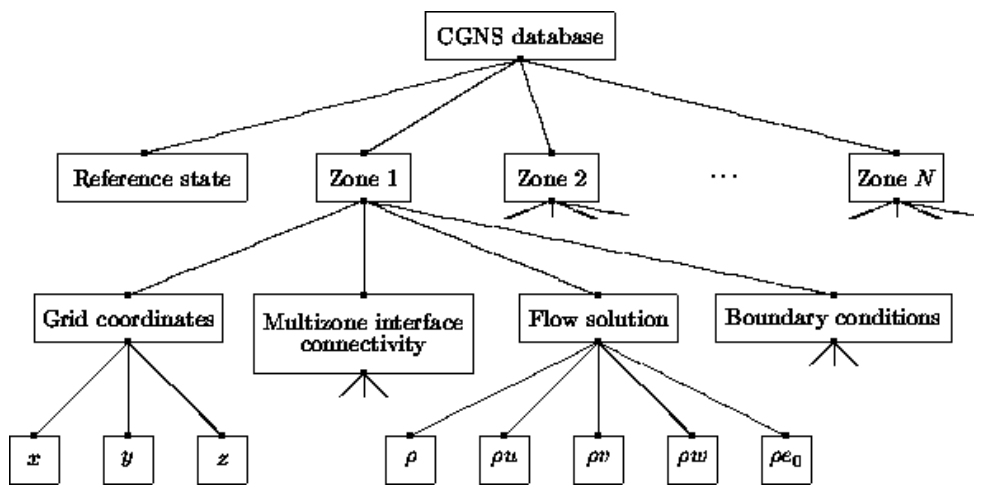
\includegraphics[width=0.6\textwidth]{img/CGNS_database_hierarchy.png}
  \caption{CGNS database hierarchy. Image from cgns.github.io}
  \label{fig:cgns-db-hierarchy}
\end{figure}

Elements are stored in sections where they are grouped by element type
in the case of SEPARATED CGNS files or all the elements are grouped
together in the case of a MIXED CGNS file. Depending on the file
format, the \texttt{InputCGNS.cpp} either uses ExtractMixedElemInfo()
or ExtractSeparatedElemInfo(). In both case, an array
\texttt{ElementConnectivity} is read in, containing the node IDs for
each element (in the MIXED format the element type must also be
specified for each element). Each function takes the
\texttt{ElementConnectivity} array and generates a vector
\texttt{elemInfo} which contains the type and node list for each
element.\\

The function ReadFaces converts from \texttt{elemInfo} into a face
representation, where each element is defined by its face
(\texttt{ElementFaces}), each face is defined by its nodes
(\texttt{FaceNodes}), and the boundary element faces of the mesh are
stored in \texttt{BndElementFaces}. These three variables are required
for the next function \texttt{ResetNodes} and allows us to re-use a
large section of code from the \texttt{InputStar} converter. \\

The final step that must be mentioned is the fact that CGNS and
NekMesh use different conventions for the order in which to list
higher order nodes. In the functions \texttt{GenElement2D} and
\texttt{GenElement3D}, we must use mappings generated by
\texttt{CGNSReordering} to map between the diffent
conventions. Although these could be produced algorithmically (and one
would want to if CGNS supported orders higher than 4th), for the
moment they have been hard-coded in by manually comparing the node
orderings in the CGNS SIDS \cite{SIDS_node_ordering} and NekMesh
\ref{sect:HO_node_ordering}.

%\subsection{CCM/CGNS shared base class (InputStarCGNS.cpp)}
%\texttt{ResetNodes} is the function responsible with renumbering the
%node IDs in accordance with the rules in section \ref{}. It requires
%the variables \texttt{ElementFaces} and \texttt{FaceNodes}, which are
%created differently in the two input modules, since .ccm and .cgns
%store elements differently.\\ \texttt{CreateElements} creates the 3D
%and then 2D elements

\section{Process Modules}
\section{Output Modules}


\begin{thebibliography}{References}
 \bibitem{NekMesh_paper} NekMesh: An open-source high-order mesh generation framework
 \bibitem{textbook} George Karniadakis, Spencer Sherwin, \textit{Spectral/hp Element Methods for Computational Fluid Dynamics}
 \bibitem{SIDS_node_ordering}\url{ https://cgns.github.io/CGNS_docs_current/sids/conv.html\#unstructgrid}
\end{thebibliography}

% \end{document}
